\chapter{The enriched B\'ezier dual basis}
\label{chp:chapter4}
\graphicspath{{figures/}{figures/chapter4/}}
\pgfplotsset{
    table/search path={{figures/chapter4/data},{data}},
}
\externaldocument[iii-]{exampleFiles/chapter3}
\externaldocument[ii-]{exampleFiles/chapter2}

In the previous chapter, we studied the approximation power of the \Bezier dual basis and the cause of their sub-optimality is the lack of polynomial reproduction. The sub-optimality of the \Bezier dual basis deteriorates the finite element approximation when is used as the discretization of Lagrange multiplier. The development of dual basis functions that are able to reproduce higher order polynomials while maintain compact support is crucial for the implementation of the dual mortar formulation in the previous chapter.\par

Dual functional of splines was first introduced by de Boor and Fix~\cite{de1973spline} to develop a quasi-interpolation operator for splines. Later on, de Boor presented dual basis functions in~\cite{de1975local}. Thomas et al.~\cite{thomas2015bezier} introduced the \Bezier projection operator as an efficient replacement of global $L^2$ projection. The dual basis induced by \Bezier projection operator has been utlized in~\cite{MIAO2018273,zou2018isogeometric} for alleviating locking and patch coupling, correspondingly. In the finite element framework, the construction of dual basis function with optimal appxoimation power was first presented in~\cite{oswald2001polynomial}. In~\cite{lamichhane2002higher}, Lamichhane and Wohlmuth introduced locally supported and continuous dual basis functions for quadratic finite elements. Later on, Lamichhane and Wohlmuth developed a group of dual basis that have the same support as the nodal finite element basis and possess adequate approximation power. Very recently, Wunderlich et al.~\cite{wunderlich2019biorthogonal} extend the formulation in~\cite{oswald2001polynomial} to the context of isogeometric analysis.\par

However, the construction algorithm in~\cite{oswald2001polynomial} calls the assembly routine twice--the first call is to construct dual basis with minimal support while the enrichment of dual basis is finished in the second call, which is inconvenient from the implementation perspective. Moreover, the condition numbers of a series of linear problems solved in~\cite{oswald2001polynomial} grow at the rate $p$, which may not be an issue for lower order basis. However, this may pollute results from higher order basis on large scale problems. \par

Based the formulation given in~\cite{oswald2001polynomial}, we propose a quadrature-free algorithm to efficiently construct enriched dual basis functions that reproduce polynomial up to a given degree. The linear systems solved in our algorithm is independent of the mesh size. Hence, there is no needs to take care of the conditioning. In addition, we utilize the enriched dual basis in the dual mortaring of $4^\text{th}$ order problems. \par

\subsection{Dual basis functions}

\subsubsection{Bernstein dual basis functions}
For a primal Bernstein basis $\mathbf{B}$, a dual basis $\hat{\mathbf{B}}$ can be formulated by simply using the inverse Gramian as
\begin{equation}
	\hat{\mathbf{B}} = \mathbf{G}^{-1}\mathbf{B}.\label{eq:global_dual}
\end{equation}
A graphical depiction of a Bernstein basis and the corresponding dual basis is shown in Figure~\ref{fig:bezier_and_its_dual}. The Bernstein dual basis $\hat{\mathbf{B}}$ has the following important properties:
\begin{itemize}
	\item{\textbf{compact support.}} The Bernstein dual basis is locally supported and each dual basis has the same support as the corresponding primal basis function, i.e., $\supp{\hat{B}_i}=\supp{{B}_i}$.
	\item{\textbf{Polynomial completeness.}} The space spanned by the dual basis is the same as the space spanned by the primal Bernstein basis, i.e., $\spn\{\hat{\mathbf{B}}\}=\spn\{\mathbf{B}\}=\mathcal{X}$.
\end{itemize}

\begin{figure}
	\center
	\includestandalone[scale=0.7]{bezier}%  
	\hspace{1cm}
	\includestandalone[scale=0.7]{bezier_dual}%     without .tex extension
	% or use \input{mytikz}
	\caption{A Bernstein basis (left) and the corresponding dual basis (right) of degree $p=2$ defined over the knot vector $\left\{0,0,0,1/3,2/3,1,1,1\right\}$. Note that each dual basis has the same support as the corresponding primal basis function.}
	\label{fig:bezier_and_its_dual}
\end{figure}

\subsubsection{B-spline dual basis functions}
For a primal B-spline basis $\mathbf{N}$, a dual basis $\hat{\mathbf{N}}$ can be formulated abstractly as
\begin{equation}
	\langle\hat{N}_i,N_j\rangle_\Omega:=\int_\Omega\hat{N}_iN_jd\Omega=\delta_{ij}.
\end{equation}
We denote the spans of ${\mathbf{N}}$ and $\hat{\mathbf{N}}$ by $\mathcal{N},\hat{\mathcal{N}}\subset\mathcal{X}$, respectively.


We can also introduce a pair of quasi-interpolation operators
\begin{equation}
	\quasii{N}u = \sum_i\langle{\hat{N}_i,u}\rangle_\Omega{N}_i\text{, and }\quasiid{N}u = \sum_i\langle{{N}_i,u}\rangle_\Omega\hat{N}_i.\label{eq:quasi-interpolation-operators}
\end{equation}
\begin{remark}
	Both $\quasii{N}$ and $\quasiid{N}$ are projection operators, i.e., for all $u\in\mathcal{N}$, $v\in\hat{\mathcal{N}}$, $\quasii{N}u=u$ and $\quasiid{N}v=v$.
\end{remark}

The construction of a B-spline dual basis with the same properties as the Bernstein dual basis, i.e., compact support and polynomial completeness, is challenging. A globally supported B-spline dual basis with polynomial completeness can be constructed using an inverse Gramian (see Equation~\eqref{eq:global_dual}). On the other hand, a locally supported B-spline dual basis which does not have polynomial completeness can be constructed using the \Bezier extraction procedure as follows:
\begin{lemma}
	$\{\hat{\mathbf{N}}\}\in\mathcal{X}$ is dual to ${\mathbf{N}}$ if and only if
	\begin{equation}
		\hat{\mathbf{N}} = \mathbf{W}^T\mathbf{R}^T\mathbf{G}^{-1}\mathbf{B}=\mathbf{W}^T\mathbf{R}^T\hat{\mathbf{B}},\label{eq:dual_basis_form}
	\end{equation}
	where the weighted assembly matrix $\mathbf{W}^T$ is a pseudo-inverse of $\mathbf{A}$, i.e., $\mathbf{W}^T\mathbf{A} = \mathbf{I}$.
\end{lemma}
\begin{proof}
	Given a basis vector in form~\eqref{eq:dual_basis_form}, its inner product with the spline basis vector is given by
	\begin{equation}
		\langle\hat{\mathbf{N}},\mathbf{N}^T\rangle_\Omega = \mathbf{W}^T\mathbf{R}^T\langle\hat{\mathbf{B}},\mathbf{B}^T\rangle_\Omega\mathbf{C}^T\mathbf{A}=\mathbf{I}.
	\end{equation}
	On the other hand, if we assume that $\{\hat{\mathbf{N}}\}\in\mathcal{X}$ is dual to ${\mathbf{N}}$, then since $\hat{N}_i=\quasii{X}\hat{N}_i=\sum_j\langle \hat{B}_j, \hat{N}_i\rangle \hat{B}_j$, we can rewrite the basis vector $\hat{\mathbf{N}}$ in terms of $\hat{\mathbf{B}}$ as
	\begin{equation}
		\hat{\mathbf{N}} = \tilde{\mathbf{W}}^T\hat{\mathbf{B}}\text{, with } \tilde{W}_{i,j} = \langle{\hat{B}_i,\hat{N}_j}\rangle_\Omega.
	\end{equation}
	Hence, one can rewrite $\hat{\mathbf{N}}$ in form~\eqref{eq:dual_basis_form}, with $\mathbf{W}=\mathbf{C}\tilde{\mathbf{W}}$.
\end{proof}
We can now see that the construction of a locally supported dual basis can be simplified to finding a set of banded vectors $\{\mathbf{W}_i\}_{i=0}^{n_N-1}$ such that
\begin{equation}
	\mathbf{W}_i\cdot\mathbf{A}_j=\delta_{ij}.\label{eq:biorthonormal}
\end{equation}

\section{The approximation power of dual bases}\label{sec:approximation}
In most cases, a locally constructed quasi-interpolation operator $\quasii{N}$ possesses optimal approximation power. However, without special care, the corresponding locally constructed dual quasi-interpolation operator $\quasiid{N}$ possesses sub-optimal approximation power. In fact, for any degree it usually provides an approximation accuracy of only $\mathcal{O}(h)$. This is due to the fact that the dual basis underlying $\quasiid{N}$ often lacks polynomial completeness. To demonstrate this, we approximate the global Legendre polynomials using the dual basis produced by the method described in~\cite{thomas_bezier_2015}. Figure~\ref{fig:polynomial_completeness} shows the result for a degree three dual basis over a two element domain. There are significant discrepancies between the dual basis approximations and the corresponding polynomials for all Legendre polynomials except the constant function.

\begin{figure}[ht]
	\captionsetup[subfigure]{labelformat=empty, font = footnotesize}
	\centering
	\begin{subfigure}[b]{0.24\textwidth}
		\centering
		\includestandalone[scale=.5]{Q3_p=0}
		\caption{$P_0(x)$}
	\end{subfigure}
	\begin{subfigure}[b]{0.24\textwidth}
		\centering
		\includestandalone[scale=.5]{Q3_p=1}
		\caption{$P_1(x)$}
	\end{subfigure}
	\begin{subfigure}[b]{0.24\textwidth}
		\centering
		\includestandalone[scale=.5]{Q3_p=2}
		\caption{$P_2(x)$}
	\end{subfigure}
	\begin{subfigure}[b]{0.24\textwidth}
		\centering
		\includestandalone[scale=.5]{Q3_p=3}
		\caption{$P_3(x)$}
	\end{subfigure}
	\caption{The Legendre polynomials (\protect\blueline) and the corresponding best $L^2$ approximations (\protect\redline) by $3^\text{rd}$ order B\'ezier dual basis functions defined on a two element domain. B\'ezier dual basis functions can only replicate the constant function.}
	\label{fig:polynomial_completeness}
\end{figure}

In addition to the application of the dual basis as a local functional for the quasi-interpolation operator $\quasii{N}$, the dual basis is also widely used to solve constrained finite element problems. The advantage of using a dual basis as the Lagrange multiplier is that the degrees of freedom associated with the multiplier can be locally condensed out leading to a sparse, positive-definite linear system.

However, the best finite element approximation of the Lagrange multiplier method is governed by the approximation power of the Lagrange multiplier. This means that, when a conventional dual basis is used to define the Lagrange multiplier space, the approximation power of the Lagrange multiplier does not improve as the polynomial degree is increased. In this section, we discuss the theoretical requirements that a dual basis must satisfy to improve the approximation power to a given order. \par

We first state the approximation properties of a polynomial space $\mathcal{P}$, the proof of which can be found in~\cite{brenner_mathematical_2007}.
\begin{lemma}\label{lm:bramble-hilbert}
	(Bramble-Hilbert) Let $\Omega$ be star-shaped and $Q^qu$ be the Taylor polynomial of order $q$ of $u\in{H}^{q+1}(\Omega)$, then
	\begin{equation}
		\vert{u-Q^qu}\vert_{H^k(\Omega)}\leq{}C_{bh}h^{q+1-k}\vert{u}\vert_{H^{q+1}(\Omega)},\quad{}k=\left\{0,1,\dots,q+1\right\},
	\end{equation}
	where $h$ is the diameter of $\Omega$.
\end{lemma}

\begin{assumption}\label{aspt:global_polynomial_reproduction}
	(global idempotence) The dual quasi-interpolation operator $\quasiid{N}$ preserves polynomials of degree $q$ on the entire domain, i.e.,
	\begin{equation}
		\quasiid{N}p=p,\quad\forall{}p\in\mathcal{P}^q{(\Omega)}.
	\end{equation}
\end{assumption}

\begin{assumption}\label{aspt:local_support}
	(compact support) Each dual basis function $\hat{N}_i$ is supported by at most $m$ connected elements and $\supp{{N}_i}\subset\supp{\hat{N}_i}$.
\end{assumption}

From Assumption~\ref{aspt:global_polynomial_reproduction} and Assumption~\ref{aspt:local_support}, we have the following result:
\begin{lemma}\label{lemma:local_polynomial_reproduction}
	(local idempotence) For each element $\Omega_e\subset\Omega$, there is an extension element $\hat{\Omega}_e$ comprised of a fixed number of connected elements such that
	\begin{equation}
		\left(\quasiid{N}p\right)\vert_{\Omega_e}=p,\quad\forall{}p\in\mathcal{P}^q{(\hat{\Omega}_e)}.
	\end{equation}
	\begin{proof}
		We define
		\begin{equation}
			\hat{\Omega}_e=
			\begin{cases}
				\bigcup_{i=0}^{e+m-1}\Omega_i,\quad{e-m+1<0}         \\
				\bigcup_{i=e-m+1}^{n_e-1}\Omega_i,\quad{e+m-1>n_e-1} \\
				\bigcup_{i=e-m+1}^{e+m-1}\Omega_i,\quad\text{otherwise},
			\end{cases}
		\end{equation}
		where $n_e$ is the number of elements in $\Omega$. Since each $\hat{N}_i$ is supported by at most $m$ connected elements, if $\Omega_e\subset\supp{\hat{N}_i}$, then $\supp{\hat{N}_i}\subset\hat{\Omega}_e$ and the evaluation $\langle{N_i,p}\rangle$ in~\eqref{eq:quasi-interpolation-operators} can be done in $\hat{\Omega}_e$, owing to $\supp{{N}_i}\subset\supp{\hat{N}_i}$. Hence, local polynomial preservation can be obtained from the global idempotence for polynomials.
	\end{proof}
\end{lemma}

\begin{assumption}\label{aspt:local_stability}
	(local stability) The restriction of the dual quasi-interpolation operator $\quasiid{N}$ on $\Omega_e$ is bounded, i.e.,
	\begin{equation}
		\|\quasiid{N}u\|_{H^k(\Omega_e)}\leq{}C_{st}\|u\|_{H^k(\hat{\Omega}_e)}.
	\end{equation}
\end{assumption}

Using the Bramble-Hilbert lemma, local idempotence, and local stability, we can state the convergence behavior of the dual quasi-interpolation operator $\quasiid{N}$.

\begin{theorem}
	Let $k$ and $m$ be integer indices with $0\leq{k}\leq{m}\leq{q+1}$ and $u\in{}H^m(\hat{\Omega}_e)$. Then for $0\leq{}k\leq{}m$, we have
	\begin{equation}
		\|{u-\quasiid{N}u}\|_{H^k(\Omega_e)}\leq{}C_{}h^{m-k}\|{u}\|_{H^m(\hat{\Omega}_e)}
	\end{equation}
	\begin{proof}
		$\forall{}p\in\mathcal{P}^q(\hat{\Omega}_e)$, we have
		\begin{align}
			\begin{split}
				\|{u-\quasiid{N}u}\|_{H^k(\Omega_e)}&\leq{}\|{u-p}\|_{H^k(\Omega_e)}+\|{p-\quasiid{N}u}\|_{H^k(\Omega_e)}\\
				&=\|{u-p}\|_{H^k(\Omega_e)}+\|{\quasiid{N}(p-u)}\|_{H^k(\Omega_e)}\\
				&\leq{}(1+C_{st})\|{u-p}\|_{H^k(\hat{\Omega}_e)},
			\end{split}
		\end{align}
		by choosing $p=Q^qu$, we have
		\begin{equation}
		  \|{u-\quasiid{N}u}\|_{H^k(\Omega_e)}\leq{}(1+C_{st})\|{u-Q^qu}\|_{H^k(\hat{\Omega}_e)}\leq{}C_{bh}(1+C_{st})h^{m-k}\|{u}\|_{H^m(\hat{\Omega}_e)}.
		\end{equation}
	\end{proof}
\end{theorem}
Hence, in order for the dual quasi-interpolation operator $\quasiid{N}$ to converge at a given rate $t$, $\quasiid{N}$ must preserve polynomials on the entire domain up to degree $t-1$. In addition, the compact support and local stability requirements must be satisfied. In the next section, we will construct a dual basis that satisfies Assumption~\ref{aspt:global_polynomial_reproduction} and explain how the construction procedure ensures the satisfaction of Assumption~\ref{aspt:local_support} and Assumption~\ref{aspt:local_stability}.

\begin{algorithm}
	\SetKwInOut{Input}{Input}
	\SetKwInOut{Output}{Output}

	\Input{$\{\mathbf{A}_i\}_{i=0}^{n_N-1}$}
	\Output{A set of orthonormal basis vectors $\{\mathbf{A}^\perp_i\}_{i=0}^{n_B-n_N-1}$ for the null space of $\spn\left\{\mathbf{A}_i\right\}_{i=0}^{n_N-1}$}
	\BlankLine
	$j=0$\;
	Initialize $\{\mathbf{A}^\perp_i\}_{i=0}^{n_B-n_N-1}$ with zero vectors of size $n_B$\;
	\For{$i=0,1,\dots,n_N-1$}
	{
		$nz=\text{the number of nonzero entries of }\mathbf{A}_i$\;
		\If{$nz>1$}
		{
			\For{$k=1,\dots,nz-1$}{
				Map each entry of $[{{\underbrace{1,\dots,1}_{k}}, -k}]$ to $\mathbf{A}^\perp_j$ according to the indices of the nonzero entries of $\mathbf{A}_i$\;
				normalize $\mathbf{A}^\perp_j$ by $\mathbf{A}^\perp_j = \dfrac{\mathbf{A}^\perp_j}{\vert \mathbf{A}^\perp_j \vert}$ \;
				$j=j+1$\;
			}
		}
	}
	\caption{An algorithm to compute $\{\mathbf{A}^\perp_i\}_{i=0}^{n_B-n_N-1}$ with minimum support such that $\{\{\mathbf{A}^n_i\}_{i=0}^{n_N-1}$  ,$\{\mathbf{A}^\perp_i\}_{i=0}^{n_B-n_N-1}\}$ spans $\mathbb{R}^{n_B}$.}\label{alg:kernel_basis}
\end{algorithm}

\section{Embedding polynomials into the dual basis function space}\label{sec:algorithm}

We now describe how to construct a set of enriched dual basis functions which will endow $\quasiid{N}$ with polynomial reproduction up to a given degree. The construction is a two-step procedure:
\begin{enumerate}
\item For a given assembly matrix $\mathbf{A}$, we find a set of sparse vectors $\{\mathbf{W}^\text{ini}_i\}_{i=0}^{n_N-1}$ such that $\mathbf{W}^\text{ini}_i\cdot\mathbf{A}_j=\delta_{ij}$. Its matrix form $\mathbf{W}^\text{ini}$ will be taken to be the initial guess for the assembly matrix $\mathbf{W}$ of the desired dual basis.
  \item The vectors $\mathbf{W}^\text{ini}$ are then modified by vectors $\{\mathbf{W}^\text{mod}_i\}_{i=0}^{n_N-1}$ which come from the null space of $\spn\left\{\mathbf{A}_i\right\}_{i=0}^{n_N-1}$ until the required property is fulfilled. Note that such a modification will maintain the biorthogonal relation between $\{\mathbf{W}_i\}_{i=0}^{n_N-1}$ and $\{\mathbf{A}_i\}_{i=0}^{n_N-1}$ where
\begin{equation}
	\mathbf{W}_i=\mathbf{W}^\text{ini}_i+\mathbf{W}^\text{mod}_i.
\end{equation}
\end{enumerate}

\subsection{An orthonormal basis for the space $\mathbb{R}^{n_B}$}

To facilitate the construction of the enriched dual basis, we build a set of orthonormal vectors which form a basis for $\mathbb{R}^{n_B}$. Each orthonormal vector will have minimal support, where the support of a vector is taken to be the distance between the first and last nonzero entry. Since the column vectors $\mathbf{A}_i$ of $\mathbf{A}$ are orthogonal to each other, a natural choice for this basis is given by the set of vectors comprising all of the normalized $\{\mathbf{A}_i\}_{i=0}^{n_N-1}$, denoted by $\{\mathbf{A}^n_i\}_{i=0}^{n_N-1}$, and the vectors which span the null space of $\spn\left\{\mathbf{A}_i\right\}_{i=0}^{n_N-1}$, denoted by $\{\mathbf{A}^\perp_i\}_{i=0}^{n_B-n_N-1}$. Note that the nonzero entries of any $\{\mathbf{A}_i\}_{i=0}^{n_N-1}$ are unity-valued. In addition, each row of $\mathbf{A}$ contains one unity-valued entry.

The vectors $\{\mathbf{A}^\perp_i\}_{i=0}^{n_B-n_N-1}$ can be found by constructing vectors which are orthonormal to every vector in $\{\mathbf{A}^n_i\}_{i=0}^{n_N-1}$ from $\mathbb{R}^{n_i}$, where $n_i$ is the number of nonzero entries in $\mathbf{A}^n_i$. Note that each $\mathbf{A}^\perp_i$ can be used to construct a function in $\mathcal{X}$ as
\begin{equation}
	\tilde{N}_i=\left[\mathbf{A}^\perp_i\right]^T \mathbf{CB}.\label{eq:tidle-spline-basis}
\end{equation}
Since $\{\mathbf{A}^n_i\}_{i=0}^{n_N-1}$ and $\{\mathbf{A}^\perp_i\}_{i=0}^{n_B-n_N-1}$ span the space $\mathbb{R}^{n_B}$, $\{N_i\}_{i=0}^{n_N-1}$ and $\{\tilde{N}_i\}_{i=0}^{n_B-n_N-1}$ span the space $\mathcal{X}$. Algorithm~\ref{alg:kernel_basis} can be used to efficiently construct the basis vectors $\{\mathbf{A}^\perp_i\}_{i=0}^{n_B-n_N-1}$.\par

For example, using the assembly matrix $\mathbf{A}$ shown in~\eqref{eq:assembly_matrix} as input, we can construct the following set of basis vectors with Algorithm~\ref{alg:kernel_basis}:
\begin{equation}
	\Biggl\{
	\underbrace{\begin{bmatrix} 1\\ 0\\ 0\\ 0\\ 0\\ 0\\ 0\\ 0\\ 0 \end{bmatrix},
		\begin{bmatrix} 0\\ 1/\sqrt{2}\\ 0\\ 1/\sqrt{2}\\ 0\\ 0\\ 0\\ 0\\ 0 \end{bmatrix},
		\begin{bmatrix} 0\\ 0\\ 1/\sqrt{3}\\ 0\\ 1/\sqrt{3}\\ 0\\ 1/\sqrt{3}\\ 0\\ 0 \end{bmatrix},
		\begin{bmatrix} 0\\ 0\\ 0\\ 0\\ 0\\ 1/\sqrt{2}\\ 0\\ 1/\sqrt{2}\\ 0 \end{bmatrix},
		\begin{bmatrix} 0\\ 0\\ 0\\ 0\\ 0\\ 0\\ 0\\ 0\\ 1 \end{bmatrix}}_{\{\mathbf{A}^n_i\}_{i=0}^{n_N-1}},
	\underbrace{\begin{bmatrix} 0\\ 1/\sqrt{2}\\ 0\\ -1/\sqrt{2}\\ 0\\ 0\\ 0\\ 0\\ 0 \end{bmatrix},
		\begin{bmatrix} 0\\ 0\\ 1/\sqrt{2}\\ 0\\ -1/\sqrt{2}\\ 0\\ 0\\ 0\\ 0 \end{bmatrix},
		\begin{bmatrix} 0\\ 0\\ 1/\sqrt{6}\\ 0\\ 1/\sqrt{6}\\ 0\\ -2/\sqrt{6}\\ 0\\ 0 \end{bmatrix},
		\begin{bmatrix} 0\\ 0\\ 0\\ 0\\ 0\\ 1/\sqrt{2}\\ 0\\ -1/\sqrt{2}\\ 0 \end{bmatrix}}_{\{\mathbf{A}^\perp_i\}_{i=0}^{n_B-n_N-1}}
	\Biggr\}.
\end{equation}

\subsection{Constructing an initial guess $\mathbf{W}^\text{ini}_i$}
An initial guess $\mathbf{W}^\text{ini}_i$ for $\mathbf{W}$ can be constructed simply as
\begin{equation}
	\mathbf{W}^\text{ini}_i=\mathbf{A}_i/n_i,\label{eq:initial_guess}
\end{equation}
where $n_i$ is the number of nonzero entries in $\mathbf{A}_i$, since the number of nonzero entries in $\mathbf{A}_i$ is the same as that in $\mathbf{A}^n_i$ As will be seen in the next section, this initial guess is critical for finding an appropriate $\mathbf{W}^\text{mod}$ with the desired properties.

\subsection{Polynomial preservation}
We now establish an appropriate $\mathbf{W}^\text{mod}$ such that the quasi-interpolation operator $\quasiid{N}$ preserves a polynomial vector $\mathbf{P}=\left[{1, \xi,\dots,\xi^q}\right]^T$ ($q\leq{}p$). In other words,
\begin{equation}
	\quasiid{N}(\mathbf{P})=\mathbf{P}.\label{eq:global_polynomial_reproduction}
\end{equation}
Since both the dual basis function space $\hat{\mathcal{N}}$ and the polynomial space are subspaces of the piecewise Bernstein space $\mathcal{X}$, Equation~\eqref{eq:global_polynomial_reproduction} can be verified through the variational problem
\begin{equation}
	\langle v,\quasiid{N}(\mathbf{P}^T)\rangle_\Omega=\langle v,\mathbf{P}^T\rangle_\Omega,\;\; \forall v\in \mathcal{X}.\label{eq:global_polynomial_reproduction_test}
\end{equation}
Replacing $\quasiid{N}$ in Equation~\eqref{eq:global_polynomial_reproduction_test} by its definition (Equation~\eqref{eq:quasi-interpolation-operators}) and expressing $v$ in Bernstein form, we have
\begin{align}
	\begin{split}
		\langle\mathbf{B},\hat{\mathbf{N}}^T\rangle_\Omega\langle\mathbf{N},\mathbf{P}^T\rangle_\Omega&=\langle\mathbf{B},\mathbf{P}^T\rangle_\Omega\\
		\mathbf{R}\mathbf{W}\langle\mathbf{N},\mathbf{P}^T\rangle_\Omega&=\langle\mathbf{B},\mathbf{P}^T\rangle_\Omega\\
		\mathbf{W}^\text{ini}\langle\mathbf{N},\mathbf{P}^T\rangle_\Omega+\mathbf{W}^\text{mod}\langle\mathbf{N},\mathbf{P}^T\rangle_\Omega&=\mathbf{C}\langle\mathbf{B},\mathbf{P}^T\rangle_\Omega
	\end{split}
\end{align}
where the vector form of the B-spline basis $\mathbf{N}$ may be replaced by its \Bezier extraction form, i.e.,
\begin{equation}
	\mathbf{W}^\text{ini}\mathbf{A}^T\mathbf{C}\langle\mathbf{B},\mathbf{P}^T\rangle_\Omega+\mathbf{W}^\text{mod}\mathbf{A}^T\mathbf{C}\langle\mathbf{B},\mathbf{P}^T\rangle_\Omega=\mathbf{C}\langle\mathbf{B},\mathbf{P}^T\rangle_\Omega.\label{eq:splited_global_polynomial_reproduction_test}
\end{equation}
Using the initial guess defined in Equation~\eqref{eq:initial_guess} we have
\begin{equation}
	\mathbf{W}^\text{ini}\mathbf{A}^T=\mathbf{A}^n{\mathbf{A}^n}^T,
\end{equation}
where $\mathbf{A}^n$ is the matrix form of $\{\mathbf{A}^n_i\}_{i=0}^{n_N-1}$. The operator $\mathbf{A}^n{\mathbf{A}^n}^T\colon\mathbb{R}^{n_B}\rightarrow\spn\{\mathbf{A}^n_i\}_{i=0}^{n_N-1}$ is an $l^2$-projection operator for any vector in $\mathbb{R}^{n_B}$. Hence, owing to the direct sum decompostion
\begin{equation}
	\mathbb{R}^{n_B}=\spn\{\mathbf{A}^n_i\}_{i=0}^{n_N-1}\oplus\spn\{\mathbf{A}^\perp_i\}_{i=0}^{n_B-n_N-1},
\end{equation}
Equation~\eqref{eq:splited_global_polynomial_reproduction_test} is equivalent to
\begin{equation}
	\mathbf{W}^\text{mod}\mathbf{A}^T\mathbf{C}\langle\mathbf{B},\mathbf{P}^T\rangle_\Omega=\mathbf{A}^\perp{\mathbf{A}^\perp}^T\mathbf{C}\langle\mathbf{B},\mathbf{P}^T\rangle_\Omega,
\end{equation}
where $\mathbf{A}^\perp$ is the matrix form of $\{\mathbf{A}^\perp_i\}_{i=0}^{n_B-n_N-1}$, or
\begin{equation}
	\left[\mathbf{A}^\perp_i\right]^T\mathbf{W}^\text{mod}\langle\mathbf{N},\mathbf{P}^T\rangle_\Omega = \left[\mathbf{A}^\perp_i\right]^T\mathbf{C}\langle\mathbf{B},\mathbf{P}^T\rangle_\Omega=\langle \tilde{N}_i,\mathbf{P}^T\rangle_\Omega,\;\; i\in\left\{0,1,\dots,n_B-n_N-1\right\}. \label{eq:final_global_polynomial_reproduction}
\end{equation}

\begin{remark}
	Obviously, $\mathbf{A}^\perp{\mathbf{A}^\perp}^T\colon\mathbb{R}^{n_B}\rightarrow\spn\{\mathbf{A}^\perp_i\}_{i=0}^{n_B-n_N-1}$ is an $l^2$-projection operator in $\mathbb{R}^{n_B}$ with unity norm $\|\mathbf{A}^k{\mathbf{A}^k}^T\|=1$. Additionally, vectors $\{\mathbf{W}_i^\text{mod}\}_{i=0}^{n_N-1}\in\spn\{\mathbf{A}^\perp_i\}_{i=0}^{n_B-n_N-1}$, which ensures that the modification made by $\mathbf{W}^\text{mod}$ will not influence the biorthogonal relation between $\mathbf{W}$ and $\mathbf{A}$.
\end{remark}



We now develop an efficient algorithm to compute a modification matrix $\mathbf{W}^\text{mod}$ that satisfies Equation~\eqref{eq:final_global_polynomial_reproduction}. The resulting modification matrix will be as banded as possible and the zero entries in $\mathbf{W}^\text{mod}$ will remain zero in $\mathbf{W}$. In other words, there are no new nonzero entries introduced by the sum of $\mathbf{W}^\text{mod}$ and $\mathbf{W}^\text{ini}$.


\begin{algorithm}
	\SetKwInOut{Input}{Input}
	\SetKwInOut{Output}{Output}

	\Input{$\{\mathbf{A}^\perp_i\}_{i=0}^{n_B-n_N-1}$, polynomial degree $q$}
	\Output{$\mathbf{W}^\text{mod}$}
	\BlankLine
	Initialize $\mathbf{P}=\left[{1, \xi,\dots,\xi^q}\right]^T$\;
	Initialize $\mathbf{W}^\text{mod}=\mathbf{0}_{n_B \times n_N }$\;
	Assemble the matrix $\mathbf{C}\langle{\mathbf{B},\mathbf{P}^T}\rangle_\Omega$, $\langle{\mathbf{N},\mathbf{P}^T}\rangle_\Omega$ may then be obtained via the assembly operator $\mathbf{A}$\;
	\For{$i=0,1,\dots,n_B-n_N-1$}
	{
	$ind =\text{the index of the vector $\mathbf{A}_{ind}$ that is used to construct $\mathbf{A}^\perp_i$}$ in Algorithm~\ref{alg:kernel_basis} (shares the same nonzero entries as $\mathbf{A}^\perp_i$)\;
	Find $q+1$ indices $\left\{{n_0,n_1,\dots,n_{q}}\right\}$ that are closest to $ind$ and $0\leq{}n_0\leq{}n_q\leq{}n_N-1$\;
	Define a square matrix $\mathbf{M}$ from the $\left\{{n_0,n_1,\dots,n_{q}}\right\}$ columns of $\langle{\mathbf{P},\mathbf{N}^T}\rangle_\Omega$\;
	Construct a vector $\mathbf{F}=\langle \mathbf{P}, \tilde{N}_i \rangle_\Omega$ from $\mathbf{C}\langle{\mathbf{B},\mathbf{P}^T}\rangle_\Omega$ and Equation~\eqref{eq:tidle-spline-basis}\;
	Solve $\mathbf{X}=\mathbf{M}^{-1}\mathbf{F}$\;
	\For{$j=0,1,\dots,q$}
	{
		$\mathbf{W}^\text{mod}_{n_j}=\mathbf{W}^\text{mod}_{n_j}+x_j\mathbf{A}^\perp_i$\;
	}
	}
	\caption{An algorithm to construct $\mathbf{W}^\text{mod}$.}\label{alg:modification_weight}
\end{algorithm}

The procedure for constructing the matrix $\mathbf{W}^\text{mod}$ is given in Algorithm~\ref{alg:modification_weight}. The functions that are involved in one iteration of Algorithm~\ref{alg:modification_weight} for constructing a quadratic dual basis that reproduces quadratic polynomials are shown in Figure~\ref{fig:weight-modification-algorithm}. For a vector $\mathbf{A}^\perp_i$, one can construct a basis function $\tilde{N}_i$ of $\mathcal{X}$ by Equation~\eqref{eq:tidle-spline-basis} (Figure~\ref{fig:weight-modification-a}). Since $\mathbf{A}^\perp_i$ is constructed by $\mathbf{A}_{11}$ from Algorithm~\ref{alg:kernel_basis}, $\left[\langle\mathbf{P}, N_{10}\rangle_\Omega\right]$, $\left[\langle\mathbf{P}, N_{11}\rangle_\Omega\right]$ and $\left[\langle\mathbf{P}, N_{12}\rangle_\Omega\right]$ are selected to form the matrix $\mathbf{M}$ (highlighted in Figure~\ref{fig:weight-modification-b}). A consequence of this approach is that the support of each dual basis function consists of no more than $p+q+1$ elements. Although the support is slightly enlarged through the modification procedure, it still remains local. The domain involved in the formulation of $\mathbf{M}$ is $\left[ s, e \right]$, highlighted by orange blocks. The polynomials involved in the formulation of $\mathbf{M}$ and $\mathbf{F}$ are highlighted in Figure~\ref{fig:weight-modification-c}.

\begin{figure}[ht]
	\begin{subfigure}{\linewidth}
		\center
		\includestandalone[scale=1]{tilde_spline}%     without .tex extension
		\caption{A $\tilde{N}_i$ formed by $\mathbf{A}_i^\perp$ constructed from $\mathbf{A}_{11}$ via Algorithm~\ref{alg:kernel_basis}.}\label{fig:weight-modification-a}
	\end{subfigure}
	\begin{subfigure}{\linewidth}
		\center
		\includestandalone[scale=1]{spline}%     without .tex extension
		\caption{$\left\{N_i\right\}_{i=n_0}^{n_q}$ constructed by selected $\left\{\mathbf{W}_i\right\}_{i=n_0}^{n_q}$, $s$ and $e$ are starting and ending knots of $\bigcup_{i=n_0}^{n_q}\supp{N_i}$.}\label{fig:weight-modification-b}
	\end{subfigure}
	\begin{subfigure}{\linewidth}
		\center
		\includestandalone[scale=1]{global_polynomial}%     without .tex extension
		\caption{$\mathbf{P}=\left[1, \xi, \xi^2\right]^T$}\label{fig:weight-modification-c}
	\end{subfigure}
	\begin{subfigure}{\linewidth}
		\center
		\includestandalone[scale=1]{local_polynomial}%     without .tex extension
		\caption{$\mathbf{P}\circ F=\left[1, t \circ F, t^2 \circ F\right]^T$}\label{fig:weight-modification-d}
	\end{subfigure}
	% or use \input{mytikz}
	\caption{Illustration of all involved basis functions, polynomials and elements in one iteration of Algorithm~\ref{alg:modification_weight} and Algorithm~\ref{alg:modification_weight_new}. }
	\label{fig:weight-modification-algorithm}
\end{figure}

\subsection{A robust quadrature free algorithm to construct enriched dual basis functions with polynomial preservation}

Although Algorithm~\ref{alg:modification_weight} builds locally supported dual basis functions that preserve polynomials, the use of polynomials defined on the entire domain $\left[0, 1 \right]$ in Equation~\eqref{eq:global_polynomial_reproduction} can be troublesome due to near linear dependencies that can develop as the mesh is refined. The fundamental issue is illustrated in Figure~\ref{fig:weight-modification-c}. To overcome this issue, we can modify the approach to use localized polynomials in each iteration. Consider the linear map
\begin{equation}
	F=\frac{\xi-s}{e-s}\colon  \left[s, e \right]\rightarrow \left[0 , 1\right].
\end{equation}
Replacing $\mathbf{P}$ by $\mathbf{P}\circ F = \left[1, t\circ F, \dots, t^q\circ F\right]^T$ (see Figure~\ref{fig:weight-modification-d}) in Algorithm~\ref{alg:modification_weight}, both spline basis functions and $\mathbf{P}\circ F$ are refined as the mesh is refined. As a result, the condition number of $\mathbf{M}$, constructed from $\mathbf{P}\circ F$, will not deteriorate as the mesh is refined. $\mathbf{P}\circ F$ can be constructed from $\mathbf{P}$ through an affine mapping operator $\mathbf{T}$ as
\begin{equation}
	\mathbf{P}\circ F = \mathbf{T} \mathbf{P}.
\end{equation}
For the example shown in Figure~\ref{fig:weight-modification-algorithm}, the operator $\mathbf{T}$ is given by
\begin{equation}
	\mathbf{T}=
	\begin{bmatrix}
		1                              & 0                    & 0                  \\
		\dfrac{-s}{e-s}                & \dfrac{1}{e-s}       & 0                  \\
		\left(\dfrac{-s}{e-s}\right)^2 & \dfrac{-2s}{(e-s)^2} & \dfrac{1}{(e-s)^2}
	\end{bmatrix}.
\end{equation}

Hence, the two linear systems are essentially the same with the operator $\mathbf{T}$ acting as a pre-conditioner that improves the conditioning of the matrix $\mathbf{M}$ in Algorithm~\ref{alg:modification_weight}. A generalized algorithm that computes the affine mapping operator $\mathbf{T}\colon\; \mathbf{T}\mathbf{P}\circ F_1=\mathbf{P}\circ F_2$, with $F_1 = \frac{\xi-s_1}{e_1-s_1}$ and $F_2 = \frac{\xi-s_2}{e_2-s_2}$ is given in Algorithm~\ref{alg:affine_mapping}.\par

\begin{algorithm}
	\SetKwInOut{Input}{Input}
	\SetKwInOut{Output}{Output}

	\Input{The highest polynomial degree $q$, $\{s_1,e_1\}$ and $\{s_2,e_2\}$}
	\Output{Matrix form of operator $\mathbf{T}$}
	\BlankLine
	Compute $s = \dfrac{s_2-s_1}{e_1-s_1}$ and $e = \dfrac{e_2-s_1}{e_1-s_1}$\;
	Initialize $\mathbf{T}_{q\times q}$\;
	\For{$j=0,1,\dots,q$}
	{
		\For{$i=0,1,\dots,j$}
		{
			$T_{i,j}= \binom{j}{i}\frac{(-s)^{j-i}}{(e-s)^j}$
		}
	}
	\caption{An affine mapping operator $\mathbf{T}\colon\; \mathbf{T}\mathbf{P}\circ F_1=\mathbf{P}\circ F_2$.}\label{alg:affine_mapping}
\end{algorithm}

Another issue with Algorithm~\ref{alg:modification_weight} is the need to call a matrix assembly routine during the construction of the matrix $\mathbf{C}\langle{\mathbf{B},\mathbf{P}^T}\rangle_\Omega$. Leveraging the \Bezier element extraction operator, the affine mapping operator, and the closed form expression of the inner product between Bernstein basis functions and polynomials, we can develop a quadrature-free formulation for the proposed dual basis. The procedure is given in Algorithm~\ref{alg:modification_weight_new}.

\begin{algorithm}
	\SetKwInOut{Input}{Input}
	\SetKwInOut{Output}{Output}

	\Input{$\{\mathbf{A}^\perp_i\}_{i=0}^{n_B-n_N-1}$, polynomial degree $q$}
	\Output{$\mathbf{W}^\text{mod}$}
	\BlankLine
	Initialize $\mathbf{W}^\text{mod}=\mathbf{0}_{n_B \times n_N }$\;
	Initialize $\mathbf{P}=\left[{1, \xi,\dots,\xi^q}\right]^T$\;
	Initialize $\mathbf{D}=\int_0^1 \mathbf{B} \mathbf{P}^T d\xi$ by Equation~\eqref{eq:inner_product_bernstein_polynomial}\;
	\For{$i=0,1,\dots,n_B-n_N-1$}
	{
	$ind =\text{the index of the vector $\mathbf{A}_{ind}$ that is used to construct $\mathbf{A}^\perp_i$}$ in Algorithm~\ref{alg:kernel_basis} (shares the same nonzero entries as $\mathbf{A}^\perp_i$)\;
	Find $q+1$ indices $\left\{{n_0,n_1,\dots,n_{q}}\right\}$ that are the closest to $ind$ and $0\leq{}n_0\leq{}n_q\leq{}n_N-1$, and identify involved elements\;
	Construct the block diagonal matrix $\tilde{\mathbf{D}}$ from the matrix $\mathbf{D}$. The submatrices on the diagonal correspond to the inner product between Bernstein basis functions and piecewise polynomials on each element \;
	Construct $\tilde{\mathbf{T}}$ from Algorithm~\ref{alg:affine_mapping} (see Figure~\ref{fig:T-tilde}), $\tilde{\mathbf{C}}$ by restricting the extraction operator $\mathbf{C}$ to the involved elements, $\tilde{\mathbf{A}}$ by restricting the assembly operator $\mathbf{A}$ to the involved elements and B-spline basis functions, and $\tilde{\mathbf{A}}^\perp_i$ by restricting ${\mathbf{A}}^\perp_i$ to the involved elements (see Figure~\ref{fig:C_tilde_and_A_tilde})\;
	Construct $\mathbf{M}=\tilde{\mathbf{T}}^T \tilde{\mathbf{D}}^T \tilde{\mathbf{C}}^T \tilde{\mathbf{A}}$ and $\mathbf{F}=\tilde{\mathbf{T}}^T \tilde{\mathbf{D}}^T \tilde{\mathbf{C}}^T \tilde{\mathbf{A}}^\perp_i$\;
	Solve $\mathbf{X}=\mathbf{M}^{-1}\mathbf{F}$\;
	\For{$j=0,1,\dots,q$}
	{
		$\mathbf{W}^\text{mod}_{n_j}=\mathbf{W}^\text{mod}_{n_j}+x_j\mathbf{A}^\perp_i$\;
	}
	}
	\caption{A quadrature-free algorithm to construct $\mathbf{W}^\text{mod}$.}\label{alg:modification_weight_new}
\end{algorithm}

\begin{figure}[ht]
	\begin{subfigure}{\linewidth}
		\center
		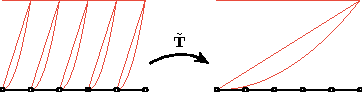
\includegraphics[scale=1.4]{algorithm_4_demo2}
		\caption{The operator $\tilde{\mathbf{T}}$ maps global polynomials to polynomials defined over the span $\left[s,e\right]$.}\label{fig:T-tilde}
	\end{subfigure}
	\begin{subfigure}{\linewidth}
		\center
		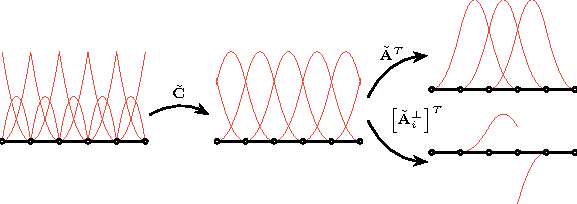
\includegraphics[scale=1.4]{algorithm_4_demo1}
		\caption{The block diagonal matrix $\tilde{\mathbf{C}}$ maps Bernstein basis functions to discontinuous B-spline basis functions, the assembly operator $\tilde{\mathbf{A}}$ constructed by restricting the operator $\mathbf{A}$ to the involved elements and spline basis functions maps discontinuous spline basis functions to continuous spline basis functions, and the operator $\tilde{\mathbf{A}}^\perp_i$ constructed by restricting the operator $\mathbf{A}^\perp_i$ to the involved elements maps discontinuous spline basis functions to functions $\tilde{N}_i$.}\label{fig:C_tilde_and_A_tilde}
	\end{subfigure}
	\caption{Illustration of the behavior of the operators used in Algorithm~\ref{alg:modification_weight_new}. }
\end{figure}

A comparison of the maximum condition numbers of the matrices $\mathbf{M}$ produced by Algorithm~\ref{alg:modification_weight} and Algorithm~\ref{alg:modification_weight_new}, respectively, for constructing $p^\text{th}$ order dual basis functions with $p^\text{th}$ order polynomial reproduction ($q=p$) is shown in Figure~\ref{fig:condition_number}. As can be seen, the condition number of $\mathbf{M}$ from Algorithm~\ref{alg:modification_weight} grows at the rate $p$, whereas the condition number of $\mathbf{M}$ from Algorithm~\ref{alg:modification_weight_new} is independent of mesh refinement. These results indicate that Algorithm~\ref{alg:modification_weight_new} has the desired robustness.

\begin{figure}[ht]
	\center
	\includestandalone[scale=1]{dual_basis_condition_number}%     without .tex extension
	% or use \input{mytikz}
	\caption{The growth of the maximum condition numbers of the matrix $\mathbf{M}$ produced by Algorithm~\ref{alg:modification_weight} and Algorithm~\ref{alg:modification_weight_new}.}
	\label{fig:condition_number}
\end{figure}

Leveraging Algorithm~\ref{alg:modification_weight} and Algorithm~\ref{alg:modification_weight_new}, the enriched dual basis reproduces global polynomials (Assumption~\ref{aspt:global_polynomial_reproduction}), and the construction process guarantees that the support of each enriched dual basis function consists of no more than $p+q+1$ elements (Assumption~\ref{aspt:local_support}). It remains to prove the local stability property (Assumption~\ref{aspt:local_stability}).

\begin{proof}[Proof of Assumption~\ref{aspt:local_stability}]
	\begin{align}
		\begin{split}
			\| \quasiid{N}u \|_{H^k(\Omega_e)} &= \| \sum_i \langle {N_i,u} \rangle_{\Omega}\hat{N}_i \|_{H^k(\Omega_e)}\\
			&\leq \| \sum_i \hat{N}_i\|_{H^k(\Omega_e)} \| \langle {\mathbf{N},u} \rangle_{\hat{\Omega}_e} \|_\infty\\
			&= \| \hat{\mathbf{N}}^T\mathbf{1} \|_{H^k(\Omega_e)} \| \langle {\mathbf{N},u} \rangle_{\hat{\Omega}_e} \|_\infty,
		\end{split}
	\end{align}
	where $\mathbf{1}$ is a unit valued vector of the same size as $\hat{\mathbf{N}}$. By rewriting $\hat{\mathbf{N}}$ in its expanded form~\eqref{eq:dual_basis_form}, we have
	\begin{equation}
		\| \quasiid{N}u \|_{H^k(\Omega_e)} \leq  \| \sum_i{B_i} \|_{H^k(\Omega_e)} \| \mathbf{G}^{-T}\mathbf{R}\mathbf{W}\mathbf{1} \|_\infty \| \langle {\mathbf{N},u} \rangle_{\hat{\Omega}_e} \|_\infty.
	\end{equation}
	From the definition of matrix norms, we then have
	\begin{equation}
		\begin{split}
			\| \quasiid{N}u \|_{H^k(\Omega_e)} &\leq \| \sum_i{B_i} \|_{H^k(\Omega_e)} \| \mathbf{G}^{-T}\mathbf{R}\mathbf{W}\|_\infty \| \langle {\mathbf{N},u} \rangle_{\hat{\Omega}_e} \|_\infty\\
			&\leq \| \sum_i{B_i} \|_{H^k(\Omega_e)} \| \mathbf{G}^{-T} \|_\infty \| \mathbf{R} \|_\infty \| \mathbf{W} \|_\infty \| \langle {\mathbf{N},u} \rangle_{\hat{\Omega}_e} \|_\infty.
		\end{split}\label{eq:proof_of_assumption3_1}
	\end{equation}
	Since the Bernstein basis forms a partition of unity over each element, we have that
	\begin{equation}
		\| \sum_i{B_i} \|_{H^k(\Omega_e)} = \| 1 \|_{H^k(\Omega_e)} = \| 1 \|_{L^2(\Omega_e)} = \sqrt{h}.\label{eq:proof_of_assumption3_2}
	\end{equation}
	Let $\mathbf{G}_{\left[ 0,1 \right]}$ be the Gramian matrix defined on the interval $\left[ 0,1 \right]$ and assume $\|\mathbf{G}^{-1}_{\left[ 0,1 \right]}\|_\infty = C_{gi}$, we have
	\begin{equation}
		\| \mathbf{G}^{-T} \|_\infty = \| \mathbf{G}^{-1} \|_\infty = h^{-1} \|\mathbf{G}^{-1}_{\left[ 0,1 \right]}\|_\infty = C_{gi}h^{-1}.\label{eq:proof_of_assumption3_3}
	\end{equation}

	Owing to the fact that the \Bezier element extraction operators are independent of the geometry and are invariant under uniform scaling, their norms are independent of the mesh size. In addition, there are a finite number of different \Bezier element extraction operators generated by uniform mesh refinement. Hence, we can assume $\|\mathbf{R}\|_\infty=C_r$. Meanwhile, thanks to Algorithm~\ref{alg:modification_weight_new}, the construction of $\mathbf{W}$ is geometry and mesh size independent. Hence, we can assume that $\|\mathbf{W}\|_\infty=C_w$.\par

	Since spline basis functions are non-negative and also form a partition of unity, from Lemma~\ref{lemma:local_polynomial_reproduction} and the Cauchy-Schwarz inequality, we have that
	\begin{equation}
		\| \langle {\mathbf{N},u} \rangle_{\hat{\Omega}_e} \|_\infty \leq \| \langle {\mathbf{1},u} \rangle_{\hat{\Omega}_e} \|_\infty = \vert \int_{\hat{\Omega}_e} u d\Omega \vert \leq \|1\|_{L^2(\hat{\Omega}_e)} \|u\|_{L^2(\hat{\Omega}_e)}=\sqrt{C_m h} \|u\|_{L^2(\hat{\Omega}_e)}\label{eq:proof_of_assumption3_4}
	\end{equation}
	where $C_m$ is the number of elements involved in $\hat{\Omega}_e$. By substituting Equations~\eqref{eq:proof_of_assumption3_2}, \eqref{eq:proof_of_assumption3_3}, and \eqref{eq:proof_of_assumption3_4} into Equation~\eqref{eq:proof_of_assumption3_1}, we have that
	\begin{equation}
		\begin{split}
			\| \quasiid{N}u \|_{H^k(\Omega_e)} &\leq C_{gi}C_wC_r \sqrt{C_m} \|u\|_{L^2(\hat{\Omega}_e)} \\
			&\leq C_{gi}C_wC_r\sqrt{C_m}\|u\|_{H^k(\hat{\Omega}_e)}.
		\end{split}
	\end{equation}
	This concludes the proof with $C_{st}=C_{gi}C_wC_r\sqrt{C_m}$.
\end{proof}
Hence, the enriched dual basis satisfies all required technical assumptions and will yield optimal approximations. Figure~\ref{fig:enriched_basis_functions} gives an example of enriched \Bezier dual basis functions of the same primal B-spline basis function with different polynomial reproduction orders. As can be seen, the approximation power is improved at the expense of the support size.

\begin{figure}[ht]
	\center
	\begin{subfigure}[t]{.45\linewidth}
		\center
		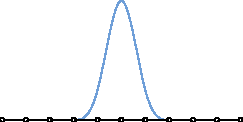
\includegraphics[width=.9\columnwidth]{p=3}
		\caption{A cubic B-spline function}\label{fig:a_cubic_spline}
	\end{subfigure}\\
	\begin{subfigure}[t]{.45\linewidth}
		\center
		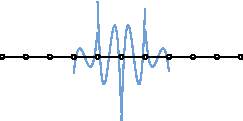
\includegraphics[width=.9\columnwidth]{p=3_c=0}
		\caption{\Bezier dual basis function of~\ref{fig:a_cubic_spline}}
	\end{subfigure}\hfil
	\begin{subfigure}[t]{.45\linewidth}
		\center
		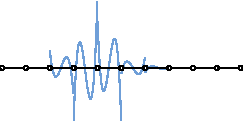
\includegraphics[width=.9\columnwidth]{p=3_c=1}
		\caption{Enriched \Bezier dual basis function of~\ref{fig:a_cubic_spline} that reproduces linear functions}
	\end{subfigure}\\
	\begin{subfigure}[t]{.45\linewidth}
		\center
		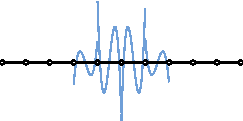
\includegraphics[width=.9\columnwidth]{p=3_c=2}
		\caption{Enriched \Bezier dual basis function of~\ref{fig:a_cubic_spline} that reproduces quadratic functions}
	\end{subfigure}\hfil
	\begin{subfigure}[t]{.45\linewidth}
		\center
		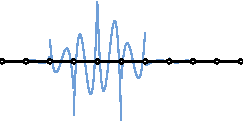
\includegraphics[width=.9\columnwidth]{p=3_c=3}
		\caption{Enriched \Bezier dual basis function of~\ref{fig:a_cubic_spline} that reproduces cubic functions}
	\end{subfigure}
	\caption{A cubic B-spline basis function and its corresponding enriched \Bezier dual basis functions with different polynomial reproduction orders. }\label{fig:enriched_basis_functions}
\end{figure}

\FloatBarrier

\section{Applications to $2^\text{nd}$ order and $4^\text{th}$ order mortar isogeometric analysis}\label{sec:dual_mortar}

The enriched dual basis functions can be used to discretize the Lagrange multiplier space in finite element dual mortar formulations. In this section, we derive dual mortar formulations for both second and fourth order problems.

\subsection{Domain decomposition for an abstract problem}

Here, we briefly recall the dual mortar method. Let $\Omega$ be a bounded domain. We decompose it into slave $\Omega_s$ and master $\Omega_m$ patches such that $\bar{\Omega}_s\cup\bar{\Omega}_m=\bar{\Omega}$ and $\Omega_s\cap\Omega_m=\emptyset$. We denote by $\partial\Omega_s / \partial\Omega_m$ the boundaries of the slave/master patch and by $\Gamma=\partial\Omega_s\cap\partial\Omega_m$ the intersection between the slave and the master patch (see Figure~\ref{fig:two_patch_domain}). We select the patch with the finer mesh as the slave patch. For the sake of simplicity, we restrict ourselves to the geometrically conforming situation where the intersection between two different patches is either empty, a vertex, or a common edge. In other words, no vertex serves as a hanging node. \par

\begin{figure}[ht]
	\center
	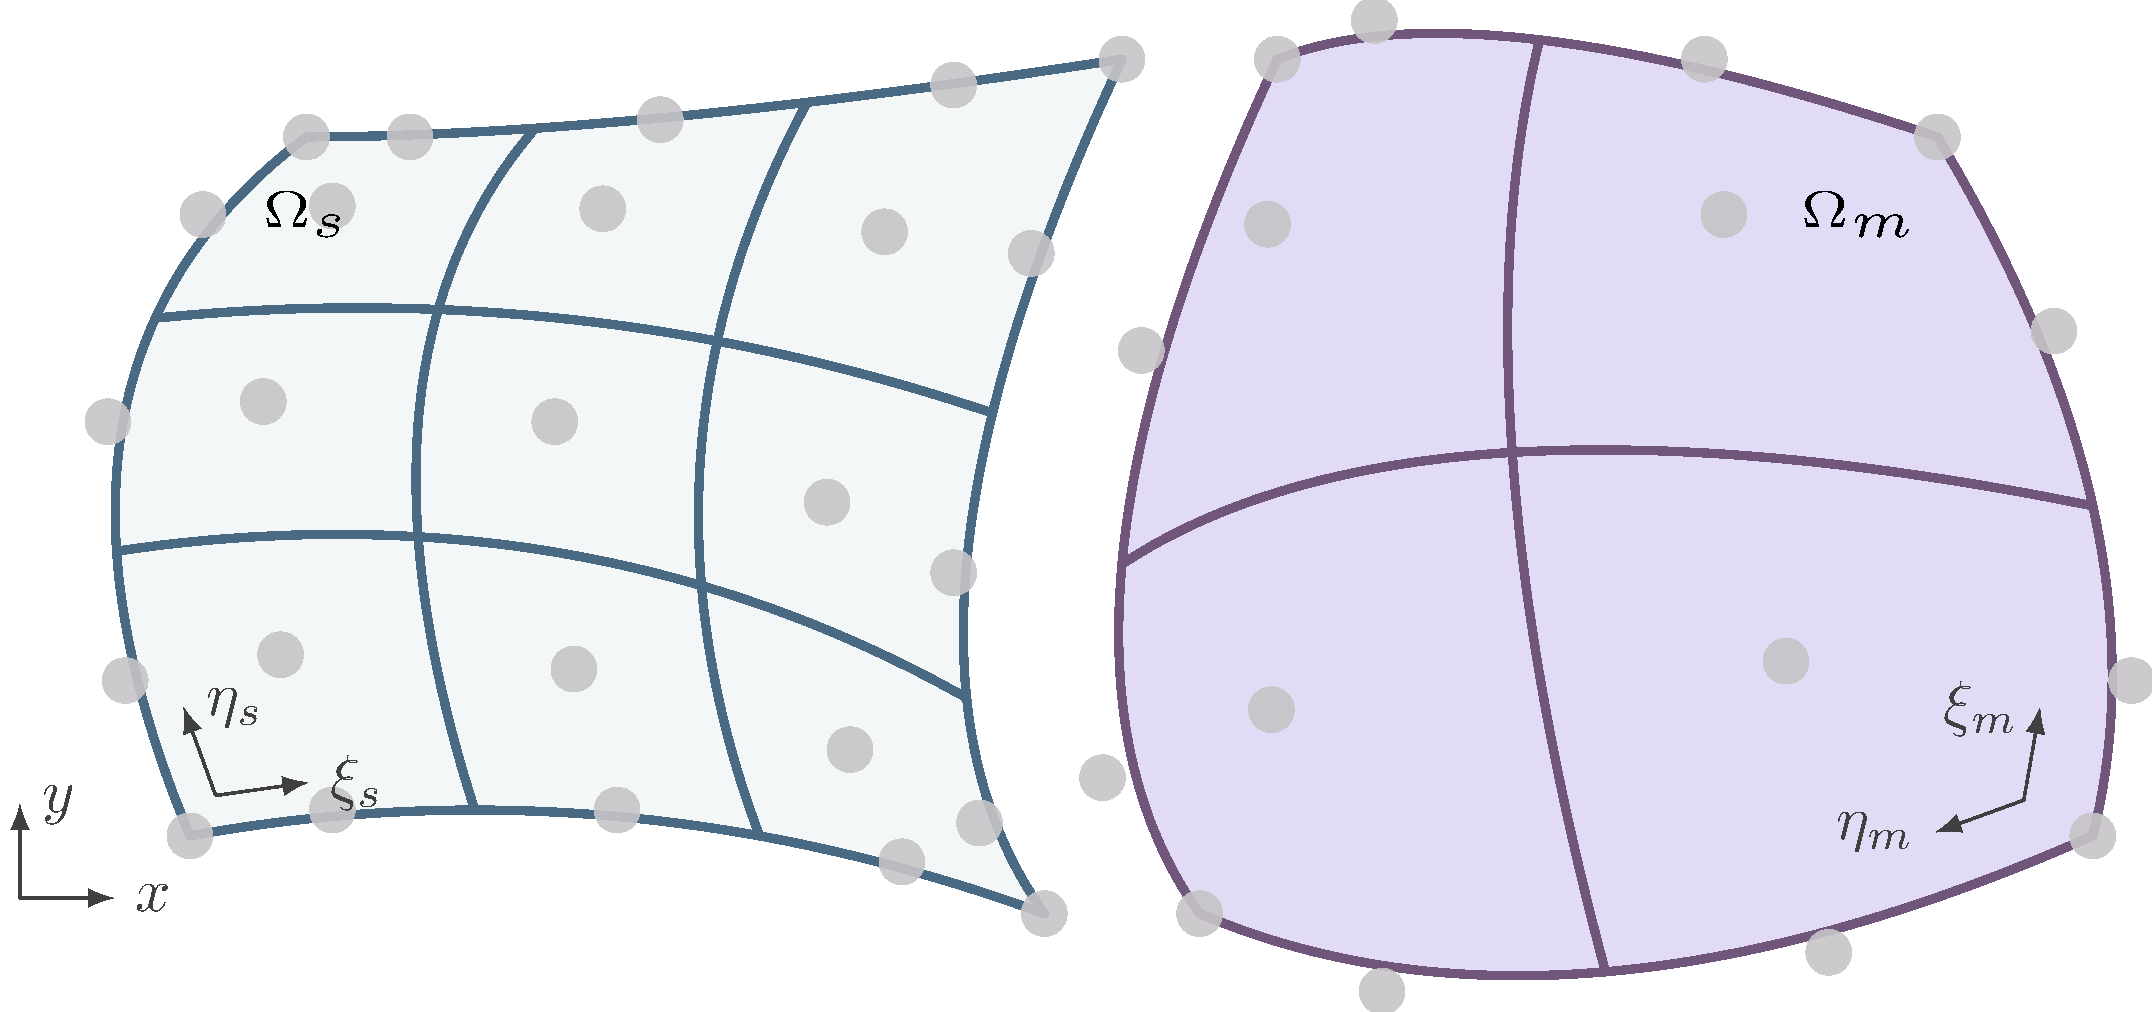
\includegraphics[width=.7\columnwidth]{two_patch_domain}
	\caption{A two-patch planar domain $\Omega$ consisting of two patches $\Omega_s$ and $\Omega_m$. }\label{fig:two_patch_domain}
\end{figure}

We consider the following abstract variational problem. Let $\mathcal{V}$ be a Hilbert space that satisfies homogeneous Dirichlet boundary conditions on $\partial \Omega$. For a given $f\in \mathcal{V}'$, find $u\in \mathcal{V}$ such that
\begin{equation}
	a(u,v)=\langle {f,v} \rangle_\Omega \quad\quad\forall v\in\mathcal{V}.\label{eq:abstract_weak_form-chapter4}
\end{equation}

In order to approximate the solution of variational problem~\eqref{eq:abstract_weak_form-chapter4} on the decomposed domain $\Omega$, $\Omega_s$ and $\Omega_m$ are discretized with non-conforming NURBS patches. The discrete spaces satisfying the homogeneous Dirichlet boundary conditions are denoted by $\mathcal{X}_s^h$ and $\mathcal{X}_m^h$, respectively. However, the function space
\begin{equation}
	\mathcal{X}^h\coloneqq \left\{ v\in L^2(\Omega) \left| \quad v\vert_{\Omega_l}\in\mathcal{X}_l^h,\quad l\in\left\{ s,m \right\} \right. \right\}
\end{equation}
is not compatible with the variational problem, as functions in $\mathcal{X}^h$ are discontinuous across the intersection.\par
One solution is to modify the variational formulation~\eqref{eq:abstract_weak_form-chapter4} so that it becomes a saddle point problem: Find $(u^h,\lambda^h)\in\mathcal{X}^h\times\mathcal{M}^h$, such that
\begin{equation}\label{eq:LM-form-chapter4}
	\left\{\begin{alignedat}{2}
		a(u^h, v^h)+b(v^h,\lambda^h)&=\langle f,v^h \rangle_\Omega\quad &&\forall{}v^h\in\mathcal{X}^h,\\
		b(u^h, \mu^h)&=0\quad &&\forall{}\mu^h\in\mathcal{M}^h,
	\end{alignedat}\right.
\end{equation}
where $b(\cdot,\cdot)$, applied weakly by the Lagrange multiplier $\lambda^h$, is an abstract constrained bilinear form and $\mathcal{M}^h$ is a Lagrange multiplier space defined on the intersection $\Gamma$. In order to recover the positive definite variational formulation~\eqref{eq:abstract_weak_form-chapter4}, Bernardi \textit{et al.}~\cite{bernardi_domain_1993} introduced the following constrained space
\begin{equation}
	\mathcal{V}^h\coloneqq \left\{ v\in \mathcal{X}^h \left| \quad b(v, \mu)=0,\quad \forall \mu\in \mathcal{M}^h \right. \right\}.
\end{equation}
Then, the saddle point problem~\eqref{eq:LM-form-chapter4} is equivalent to the minimization problem~\eqref{eq:abstract_weak_form-chapter4} on the function space $\mathcal{V}^h$. The advantage of using a dual basis with compact support to discretize the Lagrange multiplier space is that the basis functions of $\mathcal{V}^h$ are much easier to construct. In particular, all the basis functions of $\mathcal{V}^h$ have compact support. This is, in general, is not possible if the basis functions of $\mathcal{V}^h$ are constructed using traditional Lagrange multiplier spaces or a globally constructed dual basis. In the latter case, the support of a dual basis function is the entire intersection on the slave side.

We can rewrite the saddle point problem in matrix form:
\begin{equation}\label{eq:disc-LM-form-chapter4}
	\begin{bmatrix}
		\mathbf{K} & \mathbf{B}^T \\
		\mathbf{B} & \mathbf{0}
	\end{bmatrix}\begin{bmatrix}
		\mathbf{U} \\
		\mathbf{\Lambda}
	\end{bmatrix}
	=
	\begin{bmatrix}
		\mathbf{F} \\
		\mathbf{0}
	\end{bmatrix},
\end{equation}
where $\mathbf{K}$ is the discretized stiffness matrix, $\mathbf{F}$ is the discretized external force vector, $\mathbf{B}$ is the discretized constraints matrix, and $\mathbf{U}$ is a nodal vector of the displacement field $u^h \in \mathcal{X}^h$ and $\mathbf{\Lambda}$ is a nodal vector of the Lagrange multiplier field $\lambda^h \in \mathcal{M}^h$. In vector form, the basis functions of $\mathcal{V}^h$ can be written as
\begin{equation}
	\mathbf{N}^{\mathcal{V}^h} = \left[\mathbf{B}^\perp\right]^T\mathbf{N}^{\mathcal{X}^h},
\end{equation}
where $\mathbf{N}^{\mathcal{X}^h}$ are the basis functions of $\mathcal{X}^h$ in vector form. All column vectors of $\mathbf{B}^\perp$ are linearly independent and they span the null space of $\mathbf{B}$. We can further partition $\mathbf{U}$ as
\begin{equation}
	\mathbf{U}=\begin{bmatrix}
		\mathbf{U}^\text{s} \\
		\mathbf{U}^\text{m} \\
		\mathbf{U}^\text{in}
	\end{bmatrix},
\end{equation}
where the slave nodal vector $\mathbf{U}^\text{s}$ consists of all degrees of freedom that will be eliminated after static condensation, the master nodal vector $\mathbf{U}^\text{m}$ consists of all degrees of freedom on the intersection that will not be eliminated after static condensation, and the inactive nodal vector $\mathbf{U}^\text{in}$ that consists of all degrees of freedom that do not contribute to the construction of $\mathbf{B}$. The constraint can then be rewritten as
\begin{equation}
	\mathbf{B}\mathbf{U}=
	\begin{bmatrix}
		\mathbf{B}^\text{s} & \mathbf{B}^\text{m} & \mathbf{0}
	\end{bmatrix}\begin{bmatrix}
		\mathbf{U}^\text{s} \\
		\mathbf{U}^\text{m} \\
		\mathbf{U}^\text{in}
	\end{bmatrix}=\mathbf{0}.\label{eq:constraint-form-chapter4}
\end{equation}
If the Lagrange multiplier space is discretized with dual basis functions, $\mathbf{B}^\text{s}$ is the identity matrix, and the bandwidth of $\mathbf{B}^\text{m}$ depends on the support size of the dual basis functions. For a constraint matrix $\mathbf{B}$, constructed with dual basis functions with compact support, $\mathbf{B}^\text{m}$ is a sparse matrix with limited bandwidth, while global dual basis functions lead to a dense $\mathbf{B}^\text{m}$. For a $\mathbf{B}$ that takes form~\eqref{eq:constraint-form-chapter4} with $\mathbf{B}^\text{s} = \mathbf{I}$, the corresponding $\mathbf{B}^\perp$ can be obtained from
\begin{equation}
	\mathbf{B}^\perp=
	\left[\begin{array}{cc}
			-\mathbf{B}^\text{m} & \mathbf{0}                                                  \\
			\cline{1-2}
			\multicolumn{2}{c}{\multirow{2}{*}{\raisebox{-2mm}{\scalebox{1.5}{$\mathbf{I}$}}}} \\
			                     &
		\end{array}\right].\label{eq:null-space-chapter4}
\end{equation}
We then have the following linear system to solve
\begin{equation}
	\mathbf{K}^{\text{mortar}}\mathbf{U}^{\text{mortar}}=\left[\mathbf{B}^\perp\right]^T\mathbf{K}\mathbf{B}^\perp\mathbf{U}^{\text{mortar}}=\left[\mathbf{B}^\perp\right]^T\mathbf{F}\label{eq:mortar-form-discretized-chapter4}
\end{equation}
where the relationship between the mortar displacement nodal vector $\mathbf{U}^{\text{mortar}}$ and $\mathbf{U}$ is given by
\begin{equation}
	\mathbf{U}=\mathbf{B}^\perp\mathbf{U}^{\text{mortar}}.
\end{equation}
With a sparse $\mathbf{B}^\perp$ obtained from the dual basis functions with compact support, the stiffness matrix of the mortar formulation $\mathbf{K}^{\text{mortar}}$ will remain sparse.\par

The quality of the approximation engendered by $\mathbf{N}^{\mathcal{V}^h}$ depends on the discrete primal space $\mathcal{X}^h$ as well as the discrete Lagrange multiplier space $\mathcal{M}^h$. It has been shown in the previous chapter that, for $\mathcal{X}^h$ of degree $p$, an optimal discretization requires the best approximation error of $\mathcal{X}^h$ to be $\mathcal{O}(h^p)$ for $2^\text{nd}$-order problems and $\mathcal{O}(h^{p-1})$ for $4^\text{th}$-order problems, respectively. In other words, $\lambda^h\in\mathcal{M}^h$ should reproduce polynomials up to degree $p-1$ for $2^\text{nd}$-order problems and up to degree $p-2$ for $4^\text{th}$-order problems, respectively. The error associated with $\lambda^h$ is usually called the consistency error. For smooth splines, to achieve optimal accuracy while maintaining the locality of the dual basis functions in $\mathcal{V}^h$, the proposed enriched dual basis is required. \par

\subsection{Vertex modification}

For a multi-patch decomposition, at least three patches will meet at a common interior vertex and several interfaces can share this vertex as a common endpoint. If we discretize the Lagrange multiplier space with a space of the same dimension as the univariate space formed by taking the trace of the slave space along the interface, we obtain too many constraints. In this case, control points in the neighborhood of a vertex may serve as both slave and master nodes and the matrix $\mathbf{B}^\perp$ cannot be formed elegantly using~\eqref{eq:null-space-chapter4}. In addition, it has been shown in the previous chapter that $\mathcal{V}^h$ constructed from a global dual basis does not satisfy the \textit{inf-sup} condition, leading to a sub-optimal approximation error. Hence, modifications to the Lagrange multiplier space in the neighborhood of vertices are needed to relax the overly constrained linear system.\par

In general, these vertex modifications can be achieved by reducing the dimension of the Lagrange multiplier space. For second-order problems, a Lagrange multiplier space of codimension $2$ of the trace space of the slave side is sufficient to remove redundant constraints. For fourth-order problems, a Lagrange multiplier space of codimension $4$ of the trace space of the slave side is preferred. To construct an enriched dual basis of codimension $2c$, we remove the first $c$ and the last $c$ vectors in $\{\mathbf{A}_i\}_{i=0}^{n_N-1}$, leaving $\{\mathbf{A}_i\}_{i=c}^{n_N-1-c}$ a $n_N-2c$-dimensional vector space. The orthonormal vector basis of the null space of $\spn\{\mathbf{A}_i\}_{i=c}^{n_N-1-c}$ can be written as $\{\mathbf{A}^\perp_i\}_{i=0}^{n_B-n_N-1}\bigcup\{\mathbf{A}^n_i\}_{i=0}^{c-1}\bigcup\{\mathbf{A}^n_i\}_{i=n_N-c}^{n_N-1}$. Now, we can construct $\mathbf{W}^\text{ini}$ from $\{\mathbf{A}_i\}_{i=c}^{n_N-1-c}$ via~\eqref{eq:initial_guess} and assemble $\mathbf{W}^\text{mod}$ from $\{\mathbf{A}^\perp_i\}_{i=0}^{n_B-n_N-1}\bigcup$ $\{\mathbf{A}^n_i\}_{i=0}^{c-1}\bigcup\{\mathbf{A}^n_i\}_{i=n_N-c}^{n_N-1}$ with Algorithm~\ref{alg:modification_weight_new}. The resulting dual basis has $2c$ fewer dimensions than the original basis and satisfies global idempotence.

\subsection{Domain decomposition for $2^\text{nd}$-order problems}

Due to the existence of the first-order weak derivative in the weak form of $2^\text{nd}$-order problems, the constrained space $\mathcal{V}^h$ should weakly satisfy a $C^0$ continuity constraint across the interface $\Gamma$. Hence, the constrained space $\mathcal{V}^h$ for $2^\text{nd}$-order problems is given by

\begin{equation}
	\mathcal{V}^h\coloneqq \left\{ v\in \mathcal{X}^h \left|\quad \int_{\Gamma} \mu \left[ u \right] d \Gamma=0,\quad \forall \mu\in \mathcal{M}^h \right. \right\},
\end{equation}
where the Lagrange multiplier space $\mathcal{M}^h$ is two dimensions less than the trace space along the slave side of the interface. As a result, in addition to the interface nodes along the master side of the interface, the first and the last interface nodes along the slave side also serve as master nodes (see Figure~\ref{fig:2nd_order_nodes}). 
\begin{figure}[ht]
	\center
	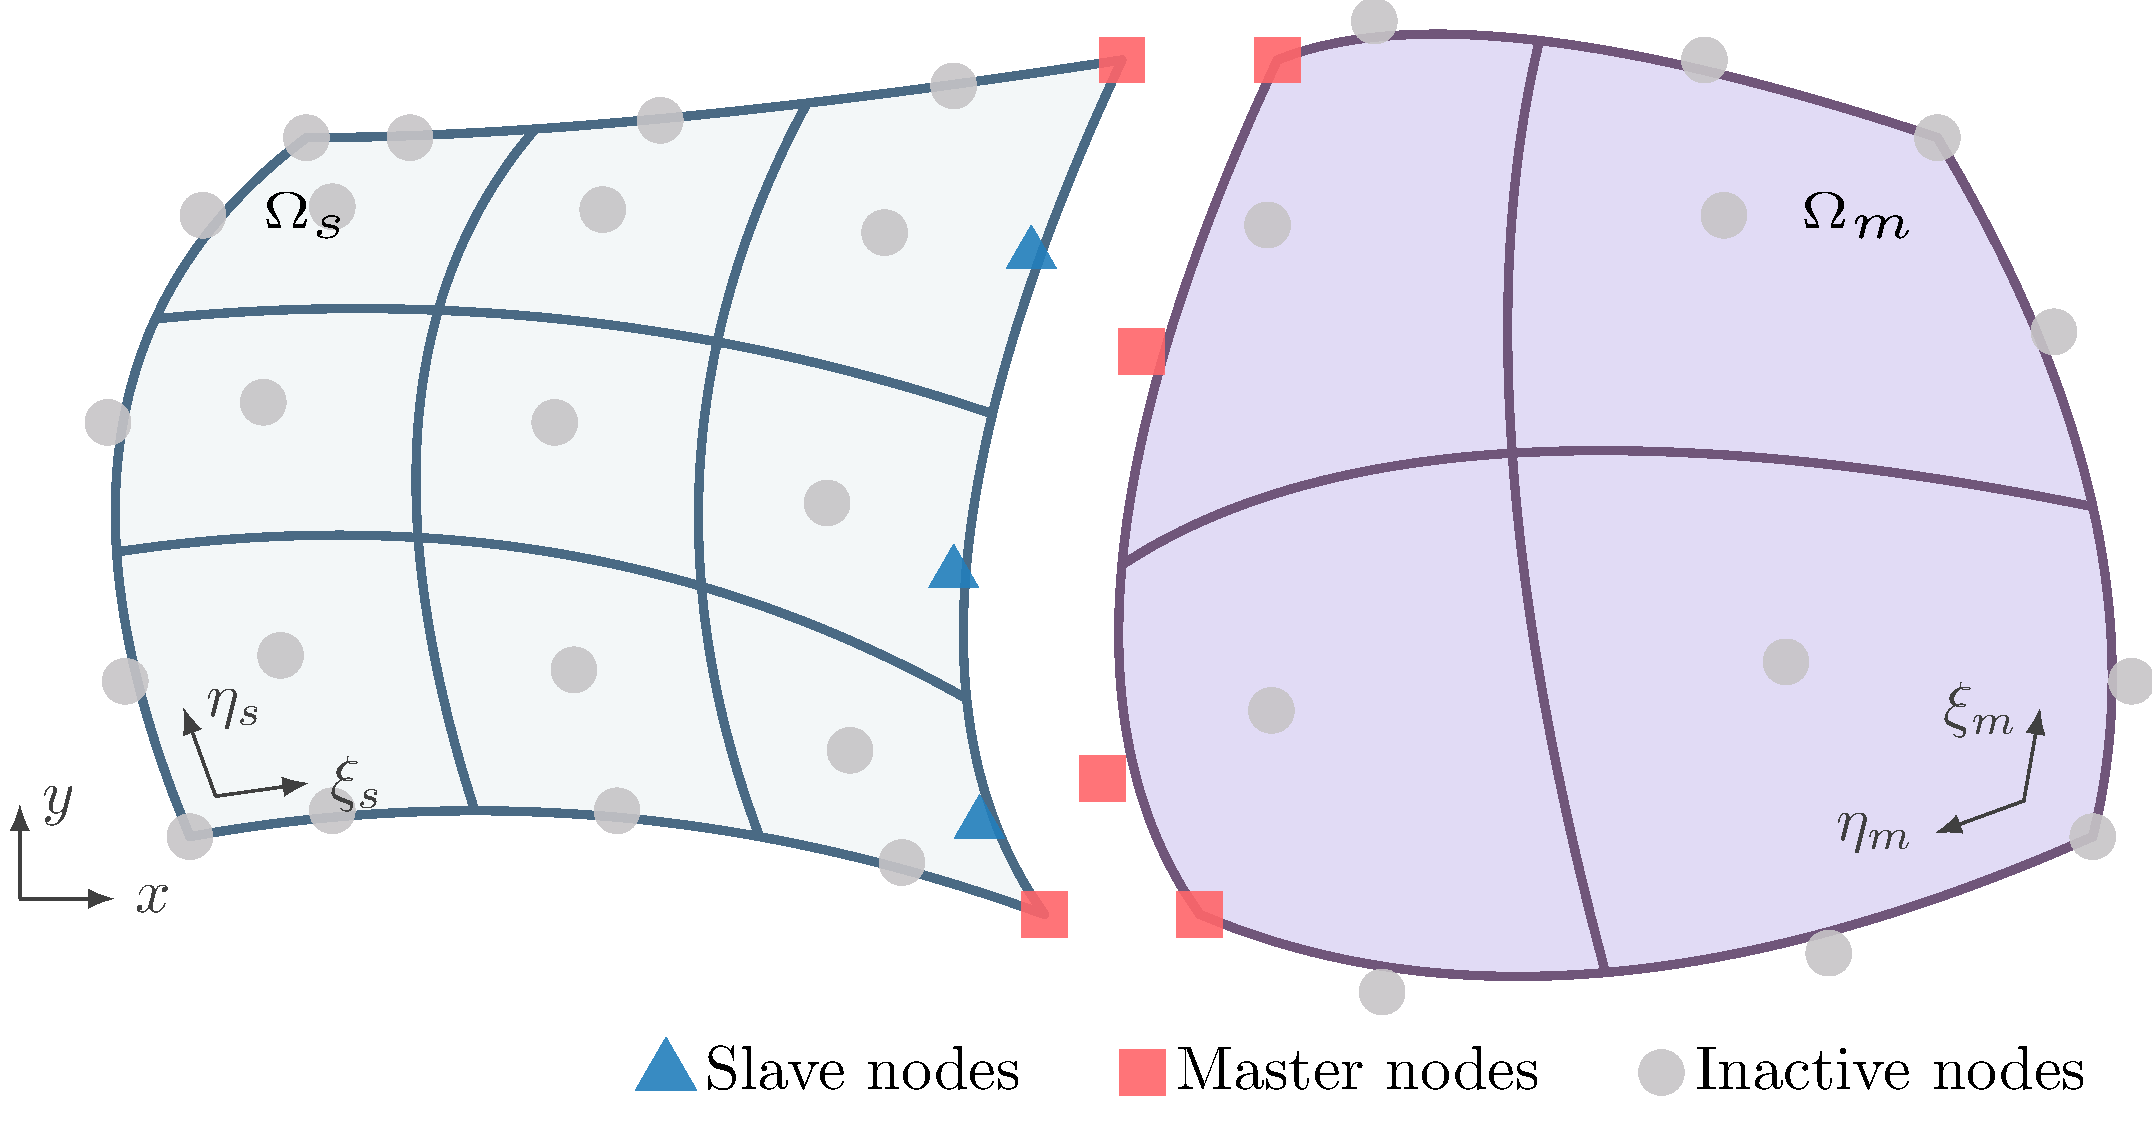
\includegraphics[width=.7\columnwidth]{two_patch_domain_poisson}
	\caption{The classification of nodes along an interface for $2^\text{nd}$-order problems. }\label{fig:2nd_order_nodes}
\end{figure}

\FloatBarrier

\subsection{Domain decomposition for $4^\text{th}$-order problems}

Due to the existence of the second-order weak derivative in the weak form of $4^\text{nd}$-order problems, the constrained space $\mathcal{V}^h$ should weakly satisfy a $C^1$ continuity constraint across the interface $\Gamma$. Hence, two Lagrange multipliers are needed to apply both a $C^0$ continuity constraint and a $C^1$ continuity constraint. The constrained space $\mathcal{V}^h$ for $4^\text{nd}$-order problems is given by

\begin{equation}\scriptstyle
	\mathcal{V}^h\coloneqq \left\{ v\in \mathcal{X}^h \left| \quad  \\\left\{\begin{alignedat}{2}
		&\int_{\Gamma} \mu_0 \left[ u \right] d \Gamma=0, &&\forall \mu_0\in \mathcal{M}_0^h\\
		&\int_{\Gamma} \mu_1 \left[ \frac{\partial u}{ \partial \xi_s} \right] d \Gamma=0\text{ if }\Gamma\parallel\eta_s\text{ or }\int_{\Gamma} \mu_1 \left[ \frac{\partial u}{ \partial \eta_s} \right] d\Gamma=0\text{ if }\Gamma\parallel\xi_s,\quad&&\forall\mu_1\in \mathcal{M}_1^h
	\end{alignedat}\right. \right. \right\},
\end{equation}
where both $\mathcal{M}_0^h$ and $\mathcal{M}_1^h$ are $4$ dimensions less than the trace space along the slave side of the interface. As a result, four nodes in the neighborhood of each vertex of $\Omega_s$ are classified as master nodes.

\begin{figure}[ht]
	\center
	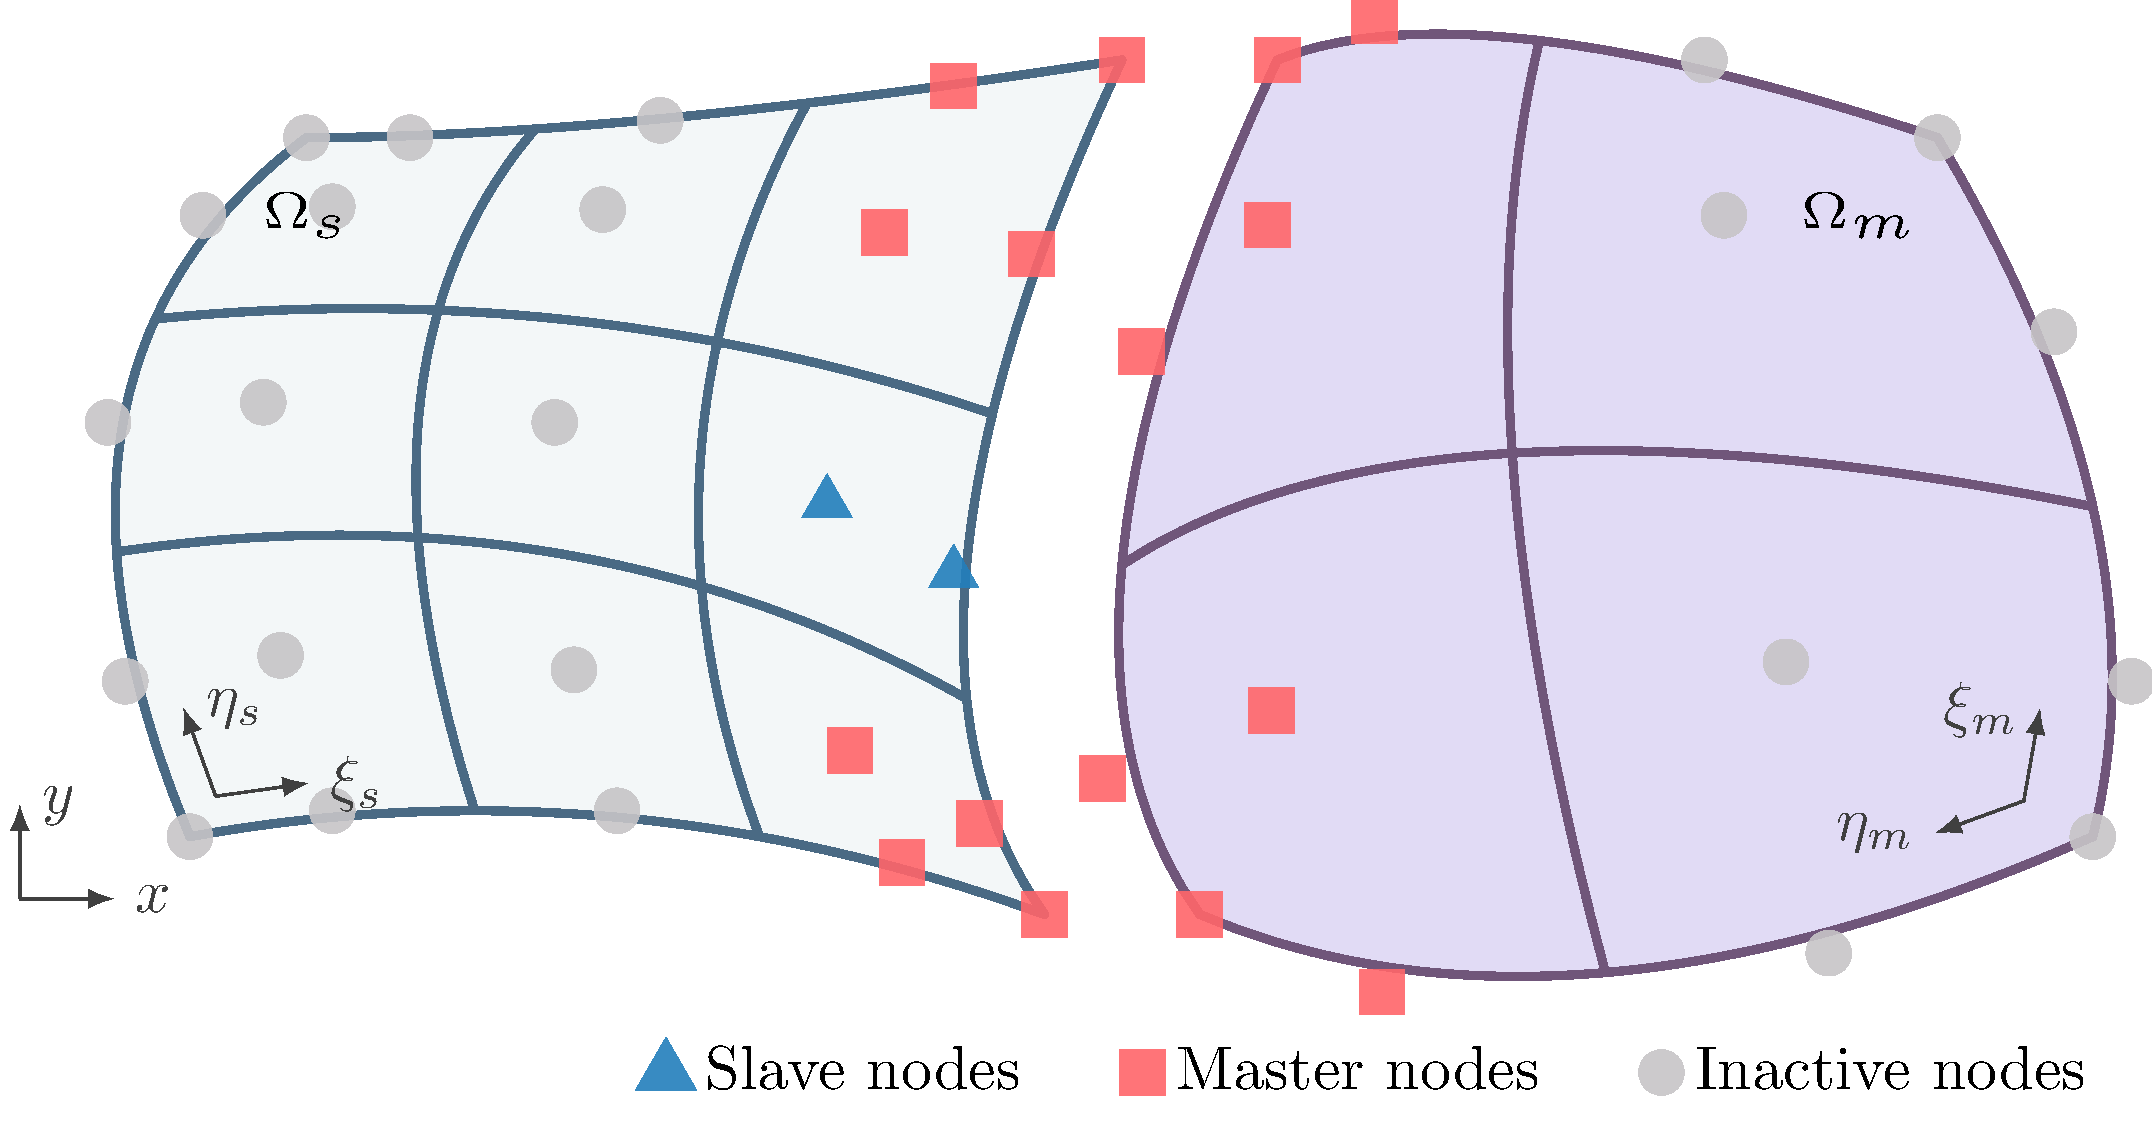
\includegraphics[width=.7\columnwidth]{two_patch_domain_biharmonic}
	\caption{The classification of nodes along an interface for $4^\text{th}$-order problems.}
\end{figure}


\section{Numerical examples}\label{sec:examples}

In this section, we investigate the performance of the enriched dual basis for several challenging second- and fourth-order benchmarks. The first example is a Poisson problem over a four-patch square domain, where the intersections are all parameterized differently. In the second problem, we model an infinite plate with a hole using four non-conforming NURBS patches. The third benchmark is a biharmonic problem over a five-patch square domain. A simply supported square Kirchhoff-Love plate is our fourth example. To verify the robustness of our enriched dual basis and dual mortar formulation for fourth-order problems, we consider the Cahn-Hilliard equation as the last benchmark. All numerical problems are solved using the Eigen library~\cite{eigenweb}. Due to the asymmetric structure of the consistent tangent matrix for the Cahn-Hilliard problem, the BiCGSTAB solver is used whereas the conjugate gradient solver is used for the rest of problems. Note that extraordinary vertices are present in all of the underlying meshes. For the \Bezier dual basis, we adopt the extraordinary vertex modification procedure described in the previous chapter.\par

Results obtained from the enriched dual basis are denoted by Enrich-$Q_i$. The performance of the enriched dual basis is compared with the global dual basis ($L^2$-$Q_i$) and the \Bezier dual basis (B\'ezier-$Q_i$). For all second-order problems, the polynomial reproduction degree $q$ is set to $p-1$ for the $p^\text{th}$-order enriched dual basis and $q=p-2$ for all fourth-order problems. These choices of degrees ensure the sparsest possible stiffness matrix while also maintaining optimality. The enriched dual bases are constructed by Algorithm~\ref{alg:modification_weight_new}.

\subsection{Poisson problem}\label{sec:poisson_problem}

We start by solving the Poisson equation $-\Delta u=f$ over the domain $\left[ 0, 1\right]\times \left[ 0, 1\right]$. The domain is decomposed into four patches, shown in Figure~\ref{fig:Poisson_mesh}. A manufactured solution is given as
\begin{equation}
	u(x,y) = \sin(2\pi x)\sin(2 \pi y).
\end{equation}
This manufactured solution satisfies the homogeneous Dirichlet boundary condition ($u=0$) and is shown in Figure~\ref{fig:Poisson_manufacture}.

\begin{figure}[ht]
	\center
	\begin{subfigure}[t]{.45\linewidth}
		\center
		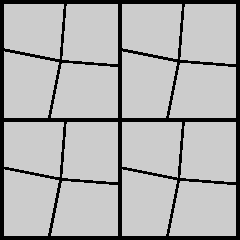
\includegraphics[scale=1.35]{four_patches_nonconform_nonmatch}
		\caption{A four-patch mesh where all intersections have both mismatched parameterizations and non-conforming meshes.}\label{fig:Poisson_mesh}
	\end{subfigure}
	\begin{subfigure}[t]{.45\linewidth}
		\center
		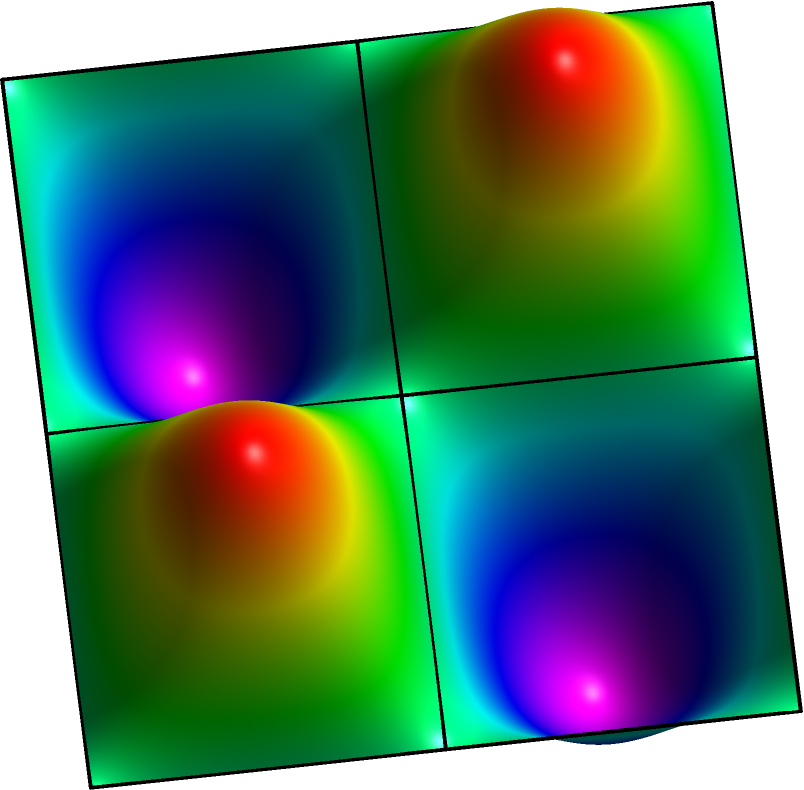
\includegraphics[scale=.41]{four_patches_solution-plot}
		\caption{A manufactured solution.}\label{fig:Poisson_manufacture}
	\end{subfigure}
	\caption{The multi-patch mesh of the domain $\Omega=\left[ 0, 1\right]\times \left[ 0, 1\right]$ and the manufactured solution that satisfies $u=0$ on $\partial\Omega$, which are utilized for the problem described in Section~\ref{sec:poisson_problem}.}
\end{figure}

Convergence plots in both the $L^2$ and $H^1$ norms are shown in Figure~\ref{fig:Poisson_convergence}. We achieve optimal convergence for the enriched dual basis for all tested polynomial degrees ($p=2,3,\ldots,5$) in both norms. For $p=2,3$, the error in the enriched dual basis is close to that of the global dual basis, whereas uniform shifts are observed for $p=4,5$. We speculate that the cause of these vertical shifts in the convergence curves is due to the non-matching parameterizations along each intersection. Since the enriched dual basis functions have a larger support size, the size of a corresponding extension element $\hat{\Omega}_e$ for the enriched dual basis will be significantly larger than that of the standard B-spline basis. As a result, the local approximation error of the enriched dual basis will be larger than that of the standard B-spline basis. The higher degree non-matching parameterizations seem to aggravate this error. However, regardless of the slight shift, the optimal convergence rates have been observed in both measures. The \Bezier dual basis, as expected, demonstrates sub-optimal convergence in both the $L^2$ and $H^1$ norms for $p=3,4,5$. In addition, in the asymptotic regime, the error increases as the polynomial degree is increased.\par

\begin{figure}[ht]
	\center
	\captionsetup[subfigure]{labelformat=empty}
	\begin{subfigure}{.45\linewidth}
		\center
		\includestandalone[scale=.8]{four_patch_poisson_L2}
	\end{subfigure}\hspace{2mm}
	\begin{subfigure}{.45\linewidth}
		\center
		\includestandalone[scale=.8]{four_patch_poisson_H1}
	\end{subfigure}
	\caption{Convergence plots for the problem described in Section~\ref{sec:poisson_problem}. On the left, error measured in the $L^2$ norm. On the right, error measured in the $H^1$ norm.}\label{fig:Poisson_convergence}
\end{figure}

Error contour plots for the cubic mesh after three global uniform refinements are shown in Figure~\ref{fig:contour_Poisson}. The contour plot of the enriched dual basis is similar to that of the global dual basis, except for small spikes in the neighborhood of extraordinary vertices. On the other hand, a significant amount of oscillatory error can be observed for the \Bezier dual basis along each intersection. Notice that the in-domain error (i.e., approximation error) is similar in all cases.

\begin{figure}
	\center
	\captionsetup[subfigure]{labelformat=empty}
	\begin{subfigure}[t]{.45\linewidth}
		\center
		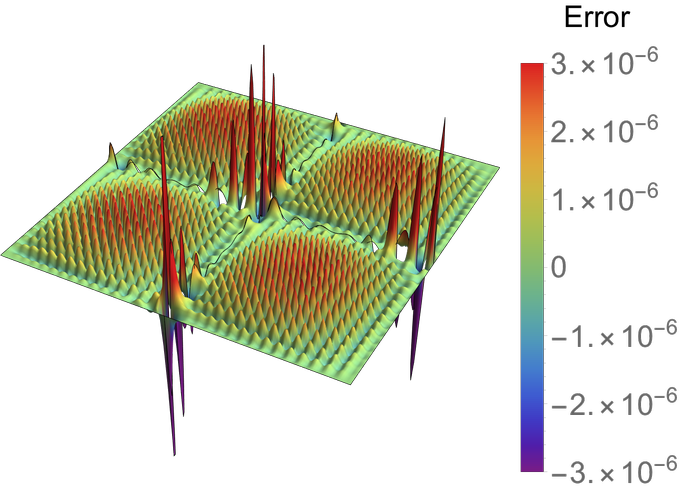
\includegraphics[scale=.52]{four_patch_poisson_op_contour}
		\caption{Enrich-$Q_3$}
	\end{subfigure}
	\begin{subfigure}[t]{.45\linewidth}
		\center
		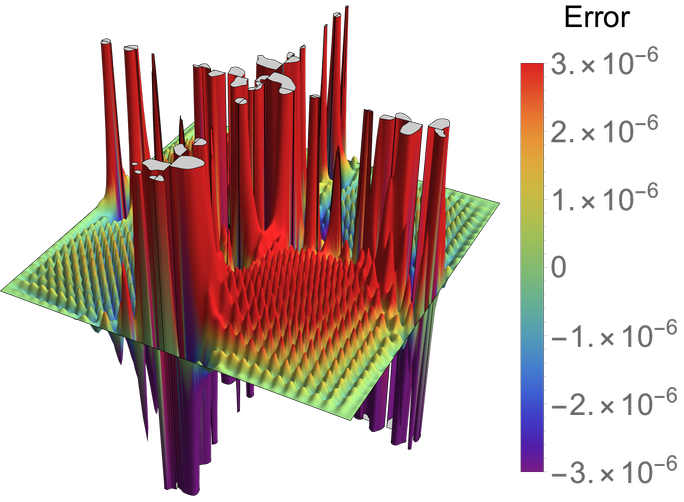
\includegraphics[scale=.52]{four_patch_poisson_Bezier_contour}
		\caption{\Bezier-$Q_3$}
	\end{subfigure}\\
	\center
	\begin{subfigure}[t]{.45\linewidth}
		\center
		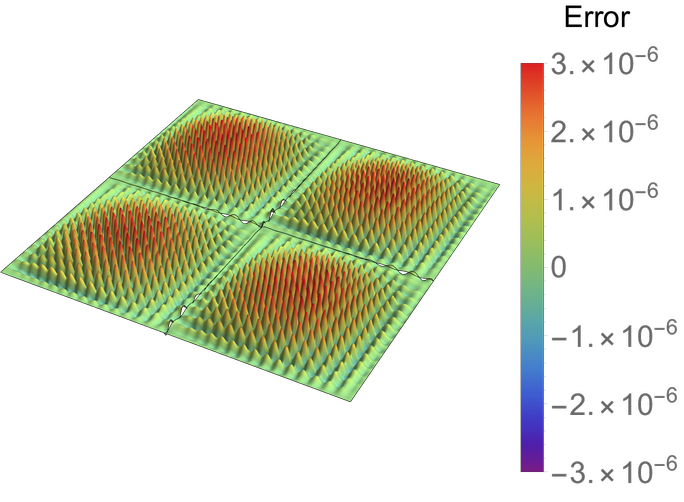
\includegraphics[scale=.52]{four_patch_poisson_L2_contour}
		\caption{$L^2$-$Q_3$}
	\end{subfigure}
	\caption{Error contour plots for the Poisson problem on a four-patch domain ($p=3$, three uniform mesh refinements). }\label{fig:contour_Poisson}
\end{figure}

\subsection{Linear elasticity -- infinite plate with a hole}\label{sec:plate_with_a_hole}

We next consider a linear elasticity problem. The problem setup and multi-patch domain are shown in Figure~\ref{fig:plate_with_hole_setup}. The traction along the outer edge is set to the exact solution

\begin{align}
	\begin{split}
		\sigma_{rr}(r,\theta)&=\dfrac{T_x}{2}(1-\dfrac{R_1^2}{r^2})+\dfrac{T_x}{2}(1-4\dfrac{R_1^2}{r^2}+3\dfrac{R_1^4}{r^4})\cos(2\theta),\\
		\sigma_{\theta\theta}(r,\theta)&=\dfrac{T_x}{2}(1+\dfrac{R_1^2}{r^2})-\dfrac{T_x}{2}(1+3\dfrac{R_1^4}{r^4})\cos(2\theta),\\
		\sigma_{r\theta}(r,\theta)&=-\dfrac{T_x}{2}(1+2\dfrac{R_1^2}{r^2}-3\dfrac{R_1^4}{r^4})\sin(2\theta).
	\end{split}
\end{align}

\begin{figure}[ht]
	\captionsetup[subfigure]{width=0.9\textwidth}
	\center
	\begin{subfigure}[t]{.3\textwidth}
		\center
		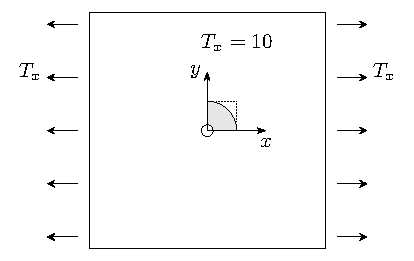
\includegraphics[scale=.7]{Platewithhole}
		\caption{Infinite plate with a hole subject to a uniaxial tension at $x=\pm \infty$.}
	\end{subfigure}
	\begin{subfigure}[t]{.3\textwidth}
		\center
		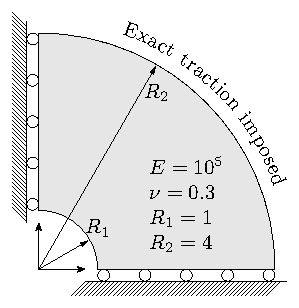
\includegraphics[scale=.7]{annular}
		\caption{The problem setup.}
	\end{subfigure}
	\begin{subfigure}[t]{.3\textwidth}
		\center
		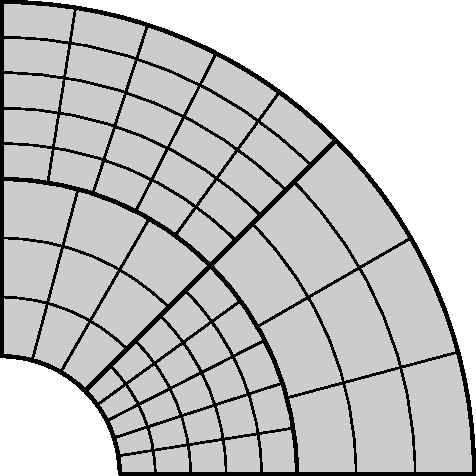
\includegraphics[scale=.45]{annular_mesh}
		\caption{The non-conforming four-patch mesh.}
	\end{subfigure}
	\caption{The infinite plate with a hole problem.}\label{fig:plate_with_hole_setup}
\end{figure}

The relative error of the displacement $\mathbf{u}$ are measured in both the $L^2$ norm and energy semi-norm
\begin{equation}
	\|\mathbf{u}-\mathbf{u}^h\|_{E}:=\sum_k\int_{\Omega_k}\frac{1}{2}\mathbf{\sigma}(\mathbf{u}-\mathbf{u}^h) \colon \mathbf{\epsilon}(\mathbf{u}-\mathbf{u}^h) d \Omega.
\end{equation}
Convergence plots for both norms are shown in Figure~\ref{fig:convergence_plate_with_hole}. Similar to the scalar Poisson problem, both the enriched and global dual basis converge optimally for all polynomial degrees in both norms. In addition, due to the absence of non-matching parameterizations along each intersection, the convergence plots of the enriched dual basis are all identical to that of the global dual basis. The convergence plots of the \Bezier dual basis are again sub-optimal.\par

\begin{figure}[ht]
	\center
	\captionsetup[subfigure]{labelformat=empty}
	\begin{subfigure}{.45\linewidth}
		\center
		\includestandalone[scale=.8]{four_patch_elasticity_L2}
	\end{subfigure}\hspace{2mm}
	\begin{subfigure}{.45\linewidth}
		\center
		\includestandalone[scale=.8]{four_patch_elasticity_energy}
	\end{subfigure}
	\caption{Convergence plots for the problem described in Section~\ref{sec:plate_with_a_hole}. On the left, the error measured in the $L^2$ norm. On the right, the error measured in the energy semi-norm.}\label{fig:convergence_plate_with_hole}
\end{figure}

Error contour plots for $p=3$ after three uniform global mesh refinements are shown in Figure~\ref{fig:contour_plate_with_hole}. The error contour plots for both the enriched and global dual basis are the same. The error in the \Bezier dual basis, however, is highly oscillatory along each intersection. Again, the in-domain errors are similar for all methods which confirms that the main contribution to the sub-optimal behavior is the consistency error.

\begin{figure}
	\center
	\captionsetup[subfigure]{labelformat=empty}
	\begin{subfigure}[t]{.45\linewidth}
		\center
		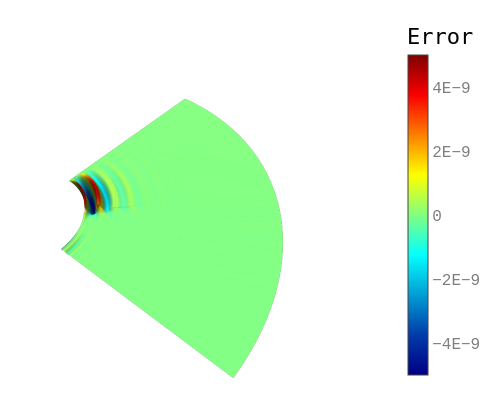
\includegraphics[scale=.4]{op_annular}
		\caption{Enrich-$Q_3$}
	\end{subfigure}
	\begin{subfigure}[t]{.45\linewidth}
		\center
		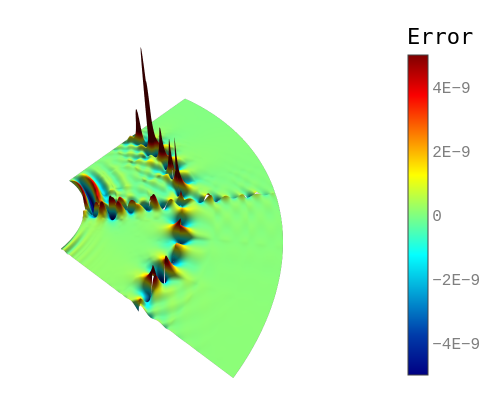
\includegraphics[scale=.4]{bezier_annular}
		\caption{\Bezier-$Q_3$}
	\end{subfigure}\\
	\center
	\begin{subfigure}[t]{.45\linewidth}
		\center
		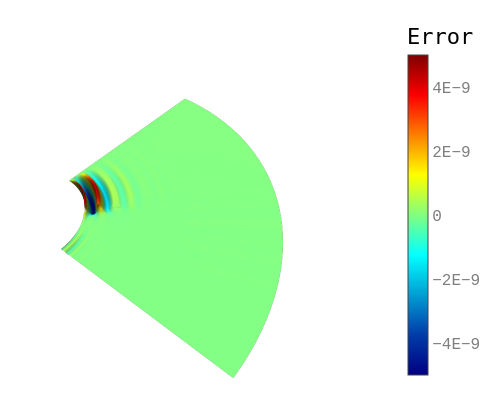
\includegraphics[scale=.4]{l2_annular}
		\caption{$L^2$-$Q_3$}
	\end{subfigure}
	\caption{Error contour plots for the linear elasticity problem on a four-patch domain ($p=3$, three uniform mesh refinements). }\label{fig:contour_plate_with_hole}
\end{figure}

\subsection{The biharmonic problem}\label{sec:biharmonic_problem}

We next consider a homogeneous biharmonic problem over the domain $\left[0, 1\right]\times \left[0, 1\right]$ and a manufactured solution
\begin{equation}
	u(x,y)=\sin(2\pi{x})^2\sin(2\pi{y})^2.
\end{equation}
The problem setup is shown in Figure~\ref{fig:biharmonic_mesh}.
\begin{figure}[ht]
	\center
	\begin{subfigure}[t]{.45\linewidth}
		\center
		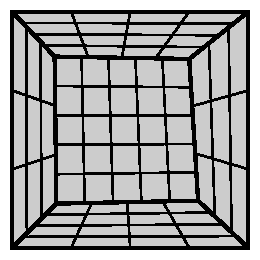
\includegraphics[scale=1.35]{five_patches_mesh}
		\caption{A non-conforming five-patch mesh.}
	\end{subfigure}
	\begin{subfigure}[t]{.45\linewidth}
		\center
		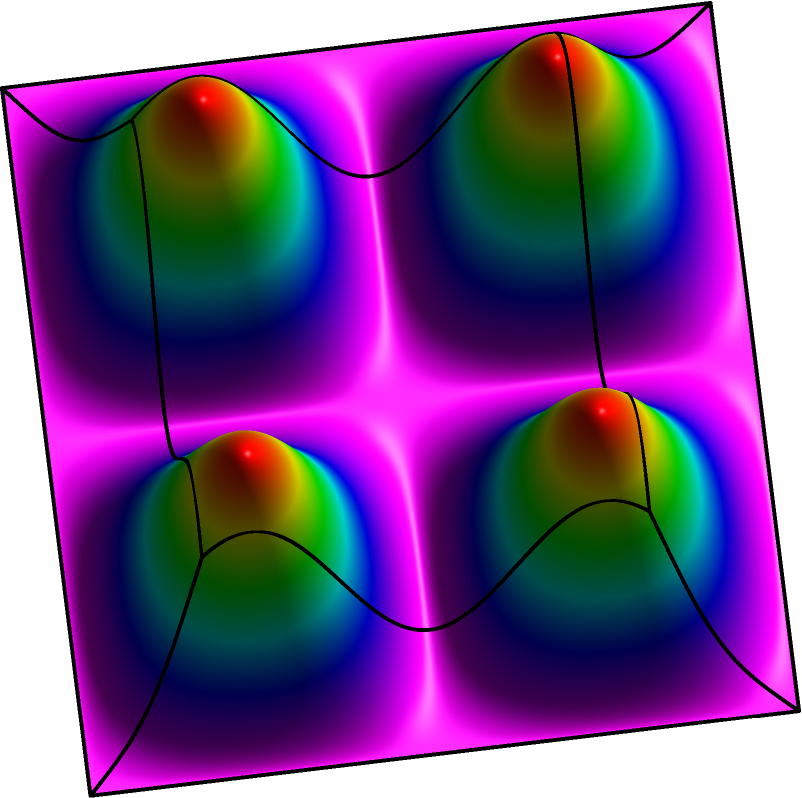
\includegraphics[scale=.425]{five_patch_solution-plot}
		\caption{A manufactured solution.}
	\end{subfigure}
	\caption{The biharmonic problem setup.}\label{fig:biharmonic_mesh}
\end{figure}

Error convergence plots for the biharmonic problem are shown in Figure~\ref{fig:convergence_biharmonic}. The enriched dual basis with $q=p-2$ produces optimal results for $p=2,3,4$ and the convergence plots are identical to those produced by the global dual basis. Note that the optimal convergence rate for quadratic basis functions is $\mathcal{O}(h^2)$ in the $L^2$ norm for biharmonic problems. For the $p=5$ case, we observe sub-optimal convergence for both the enriched and global dual basis and the most highly refined mesh in the $L^2$ norm. However, no sub-optimality is observed for the $H^2$ norm. This behavior indicates that the error occurs at certain digits of the floating point vector $\mathbf{U}^\text{mortar}$ (between the $7^\text{th}$ and $10^\text{th}$ digits for this case). We infer that the cause of this error is the poor conditioning of the stiffness matrix. In addition, previous studies~\cite{li2008effective} show that the growth rate of the condition number for the biharmonic problem is $\mathcal{O}(-h^4)$, which is huge when compared with $\mathcal{O}(-h^2)$ for the Poisson problem. This explains why the ill-conditioning of the biharmonic problem occurs much earlier than for the Poisson problem. We also attribute the slightly better performance of the enriched dual basis to their compact support and the robust construction algorithm (Algorithm~\ref{alg:modification_weight_new}). Again, the \Bezier dual basis leads to sub-optimal behavior for higher-order elements.\par

\begin{figure}
	\center
	\captionsetup[subfigure]{labelformat=empty}
	\begin{subfigure}{.45\textwidth}
		\center
		\includestandalone[scale=.8]{five_patch_biharmonic_L2}
	\end{subfigure}\hspace{2mm}
	\begin{subfigure}{.45\textwidth}
		\center
		\includestandalone[scale=.8]{five_patch_biharmonic_H2}
	\end{subfigure}
	\caption{Convergence plots for the problem described in Section~\ref{sec:biharmonic_problem}. On the left, the error measured in the $L^2$ norm. On the right, the error measured in the $H^2$ norm.}\label{fig:convergence_biharmonic}
\end{figure}

Error contour plots for the cubic mesh after two uniform refinements are shown in Figure~\ref{fig:contour_biharmonic}. Similar to second-order problems, the error contour plot for the enriched dual basis is identical to that of the global dual basis due to the absence of mismatched parameterizations along each intersection.

\begin{figure}
	\center
	\captionsetup[subfigure]{labelformat=empty}
	\begin{subfigure}[t]{.45\linewidth}
		\center
		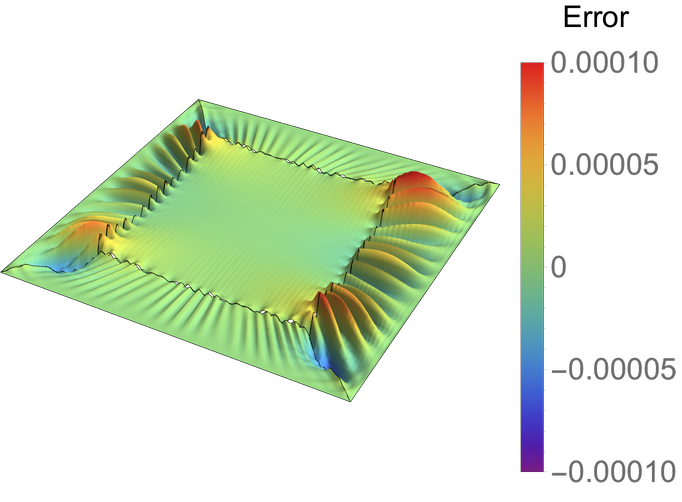
\includegraphics[scale=.52]{five_patch_biharmonic_op_contour}
		\caption{Prop-$Q_3$}
	\end{subfigure}
	\begin{subfigure}[t]{.45\linewidth}
		\center
		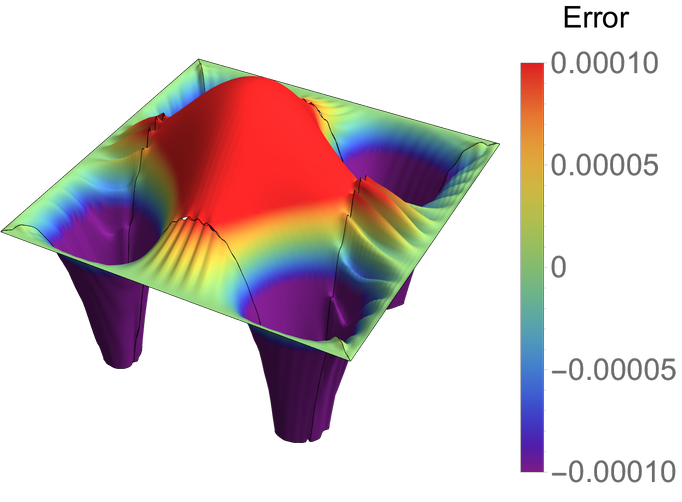
\includegraphics[scale=.52]{five_patch_biharmonic_Bezier_contour}
		\caption{\Bezier-$Q_3$}
	\end{subfigure}\\
	\center
	\begin{subfigure}[t]{.45\linewidth}
		\center
		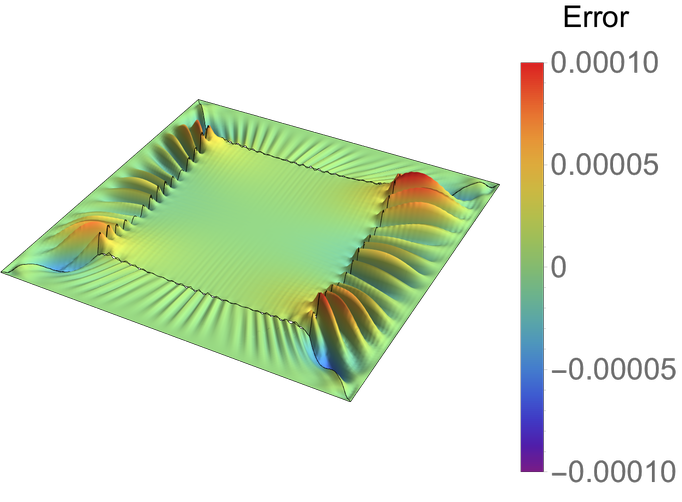
\includegraphics[scale=.52]{five_patch_biharmonic_L2_contour}
		\caption{$L^2$-$Q_3$}
	\end{subfigure}
	\caption{Error contour plots for the biharmonic problem on a five-patch domain ($p=3$, two uniform mesh refinements). }\label{fig:contour_biharmonic}
\end{figure}

\subsection{Kirchhoff plate}\label{sec:kl-plate_problem}

The last benchmark with analytical solution is a simply supported square Kirchhoff plate. The bending moments of Kirchhoff plate is given by:
\begin{equation}
	\begin{split}
		M_{xx} &= -D\left( \frac{\partial^2 w}{\partial x^2} + \nu \frac{\partial^2 w}{\partial y^2}\right),\\
		M_{yy} &= -D\left( \frac{\partial^2 w}{\partial y^2} + \nu \frac{\partial^2 w}{\partial x^2}\right),\\
		M_{xy} &= -D(1-\nu) \frac{\partial^2 w}{\partial xy},
	\end{split}
\end{equation}
where $w$ is the vertical displacement, $D = \frac{Et^3}{12(1-\nu^2)}$, $t$ is the thickness, $E$ is the Young's modulus and $\nu$ is the Poisson's ratio. The governing equation of Kirchhoff plate can be derived as
\begin{equation}
	\frac{\partial^4 w}{\partial x^4} + \frac{\partial^4 w}{\partial x^2y^2} + \frac{\partial^4 w}{\partial y^4} = \frac{q}{D}
\end{equation}
where $q$ is the pressure. In this benchmark, we consider a square plate with $L=12$ subjected to a sinusoidal presure load of
\begin{equation}
	q(x,y) = -\sin(\frac{\pi x}{L}) \sin(\frac{\pi y}{L}).
\end{equation}
We also adopt $t=0.375$, $E=4.8\times 10^5$ and $\nu = 0.38$. The analytical solution is given by
\begin{equation}
	w(x, y) = -\frac{L^4}{4D\pi^4}\sin(\frac{\pi x}{L}) \sin(\frac{\pi y}{L}).
\end{equation}
The geometry, discretization and the analytical solution of vertical displacement are shown in Figure~\ref{fig:kirchhoff_mesh}. Note that the green intersection is non-matching parameterized, whereas red curves are coupled non-comformingly. \par

\begin{figure}[ht]
	\center
	\begin{subfigure}[t]{.45\linewidth}
		\center
		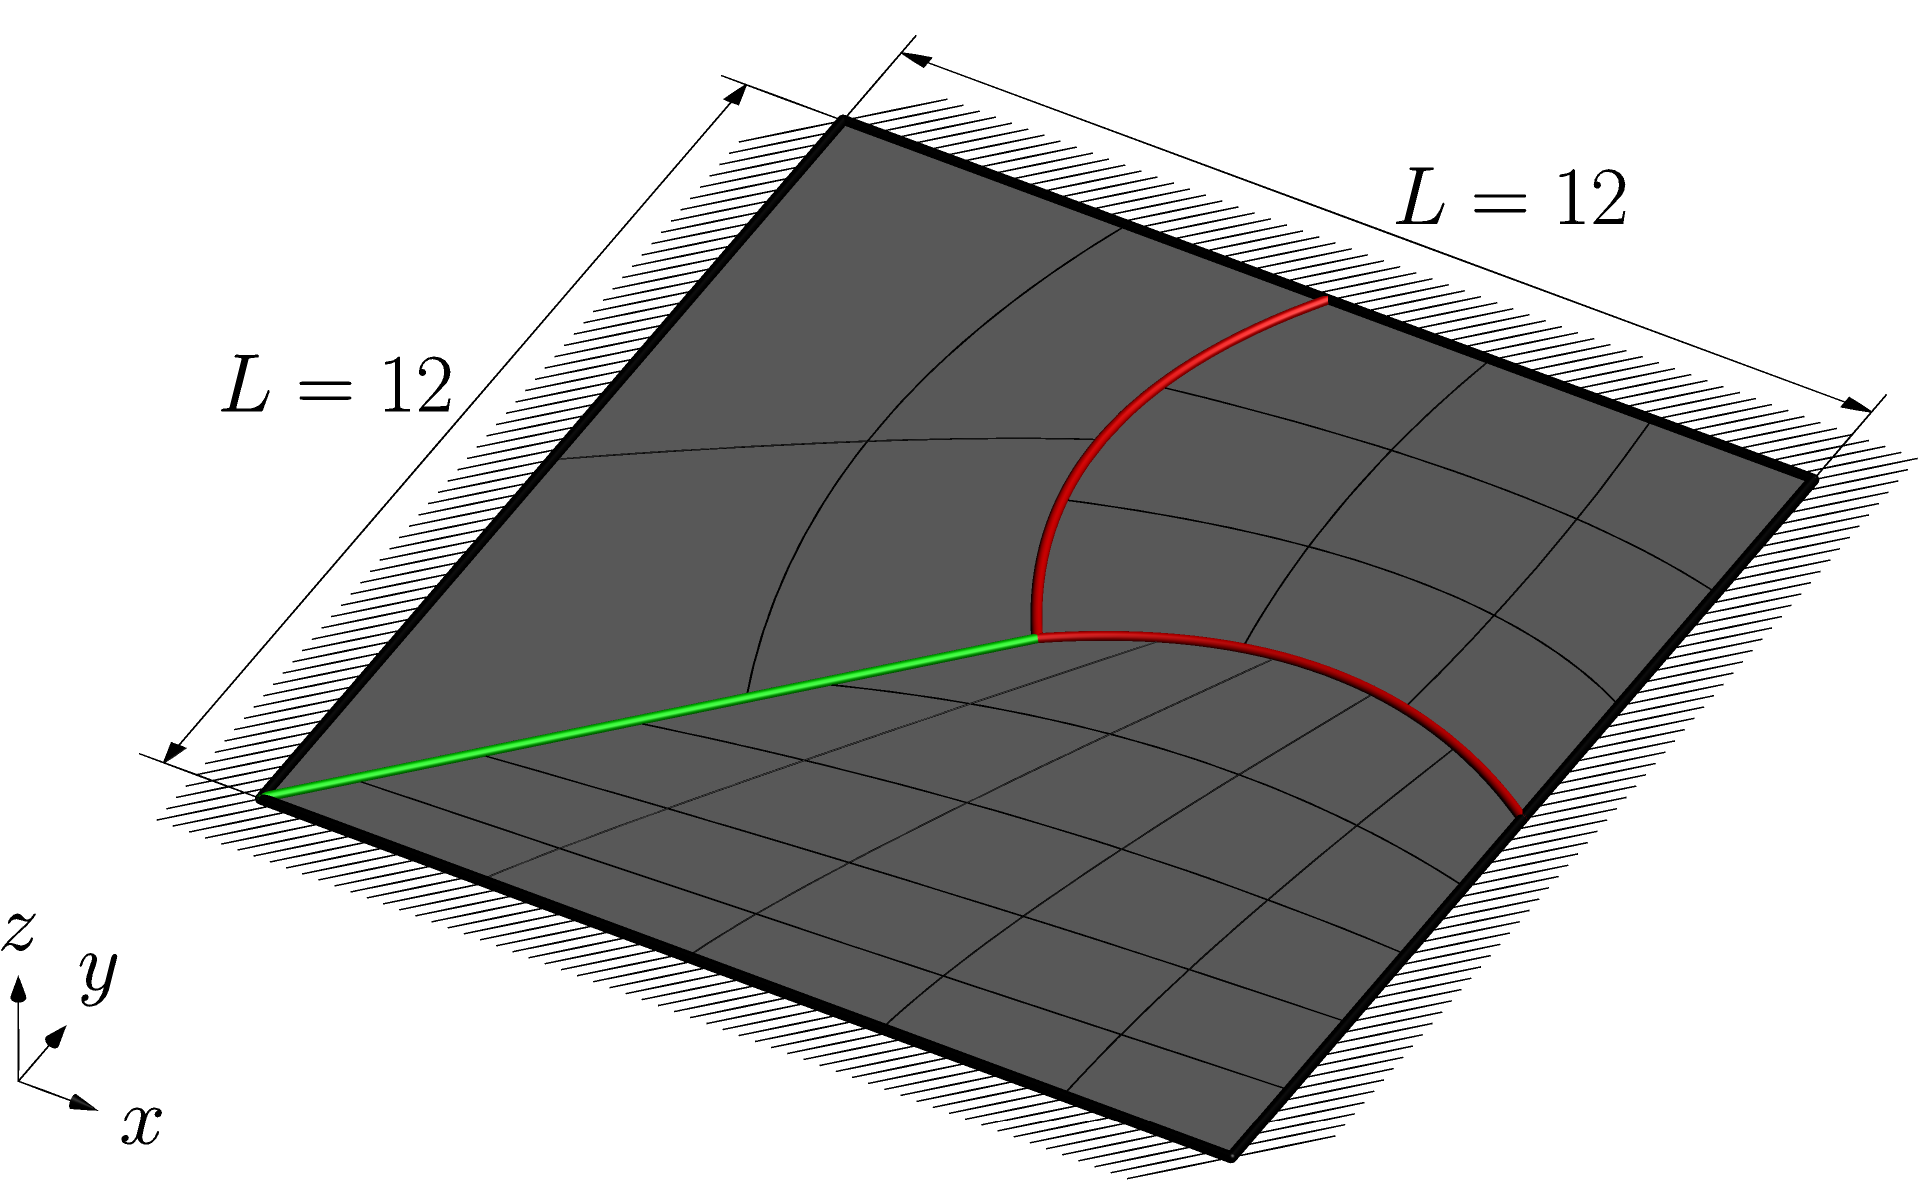
\includegraphics[scale=.4]{plate_config-plot}
		\caption{Non-matching parameterized non-conforming three-patch mesh}
	\end{subfigure}
	\begin{subfigure}[t]{.45\linewidth}
		\center
		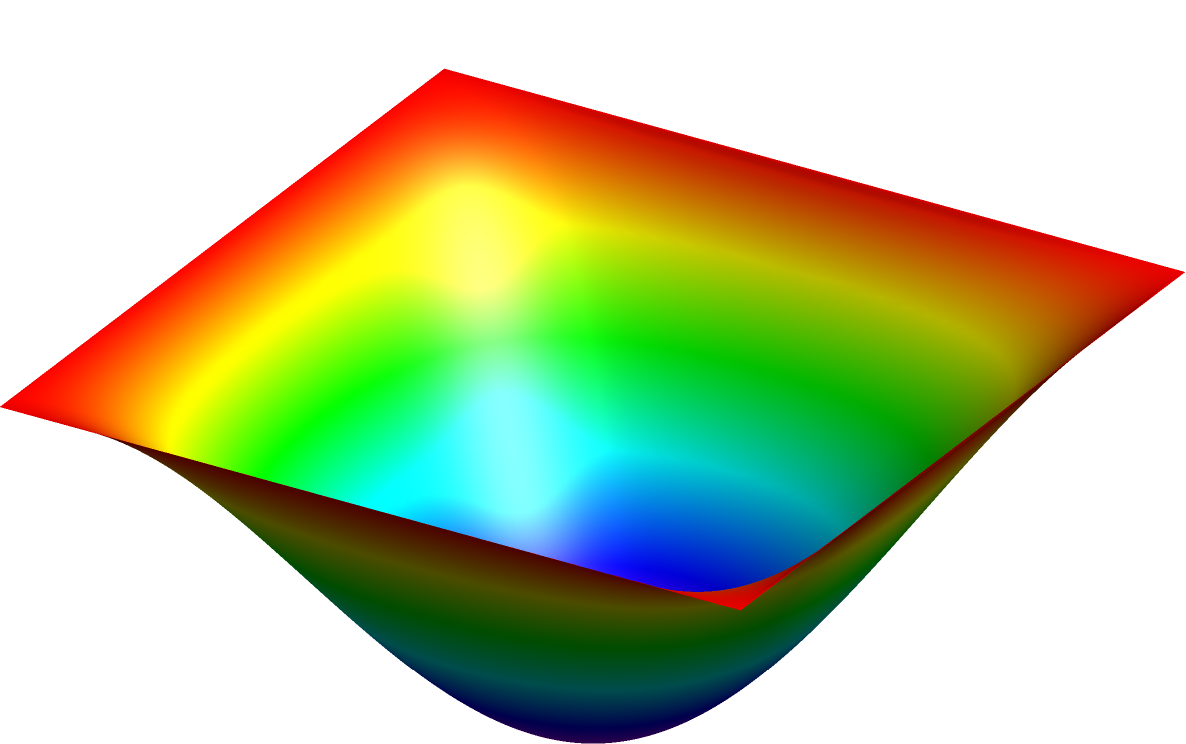
\includegraphics[scale=.3]{plate_solution-plot}
		\caption{The reference solution}
	\end{subfigure}
	\caption{The decomposition and discretization of the domain $\left[0, 1\right] \times \left[0, 1\right]$ and the refernce solution that satisfies $u=0$ on $\partial\Omega$ in Section~\ref{sec:kl-plate_problem}. The non-matching parameterized interface is denoted by green curve and the simple non-conforming discretized interfaces are denoted by red curves.}\label{fig:kirchhoff_mesh}
\end{figure}
Convergence behaviors of $w$, $M_{xx}$ and $M_{xy}$ are studied in Figure~\ref{fig:convergence_kirchhoff}. As can be seen, both the enriched dual basis and the global dual basis yield optimal results for all polynomial orders in all three measures. As the biharmonic problem, ill-conditioning at the last refinement of $p=5$ is observed in $L^2$ norm whereas convergences of errors in $M_{xx}$ and $M_{xy}$ are still optimal. Due to the presence of a non-matching parameterized intersection, vertical shifts in error plots of the enriched dual basis have been observed for higher order elements ($p = 4,5$). Again, the \Bezier dual basis generates sub-optimal results. \par

\begin{figure}[ht]
	\center
	\captionsetup[subfigure]{labelformat=empty}
	\begin{subfigure}{.45\linewidth}
		\center
		\includestandalone[scale=.8]{three_patch_plate_L2}
	\end{subfigure}\hspace{2mm}
	\begin{subfigure}{.45\linewidth}
		\center
		\includestandalone[scale=.8]{three_patch_plate_Mx}
	\end{subfigure}\\
	\begin{subfigure}{.45\linewidth}
		\center
		\includestandalone[scale=.8]{three_patch_plate_Mxy}
	\end{subfigure}
	\caption{Convergence plots for the simply supported Kirchhoff plate in Section~\ref{sec:kl-plate_problem}. Upper left: error of $w$ measured in $L^2$ norm. Upper right: error of $M_{xx}$ measured in $L^2$ norm. Bottom: error of $M_{xy}$ measured in $L^2$ norm.}\label{fig:convergence_kirchhoff}
\end{figure}

Contour plots of $\text{err}=u_x-u_x^h$ for the simply supported Kirchhoff plate problem are given in Figure~\ref{fig:contour_kirchhoff}. For the enriched dual basis and the global dual basis, no oscillation has been observed on the curved intersecitons, however, errors are evolved along the non-matching parameterized intersection. In addition, the influence of the non-matching intersection is more significant on the enriched dual basis case. For the case of the \Bezier dual basis, the consistency error is much higher and propagates into each patches.

\begin{figure}[ht]
	\center
	\captionsetup[subfigure]{labelformat=empty}
	\begin{subfigure}[t]{.45\linewidth}
		\center
		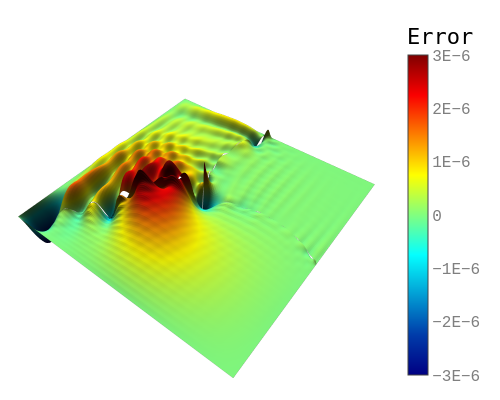
\includegraphics[scale=.4]{three_patch_plate_op_contour}
		\caption{Enrich-$Q_3$}
	\end{subfigure}
	\begin{subfigure}[t]{.45\linewidth}
		\center
		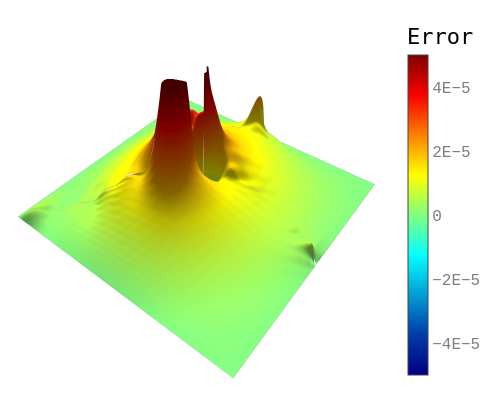
\includegraphics[scale=.4]{three_patch_plate_Bezier_contour}
		\caption{\Bezier-$Q_3$}
	\end{subfigure}\\
	\center
	\begin{subfigure}[t]{.45\linewidth}
		\center
		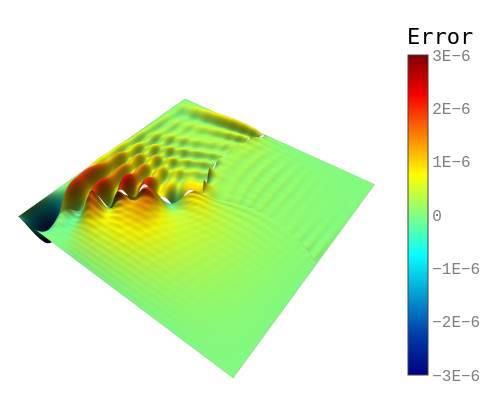
\includegraphics[scale=.4]{three_patch_plate_L2_contour}
		\caption{$L^2$-$Q_3$}
	\end{subfigure}
	\caption{Contour plots of $\text{err}=u_x-u_x^h$ for the simply supported Kirchhoff plate problem on the three-patch domain ($p=3$, and the mesh is obtained after two refinements). }\label{fig:contour_kirchhoff}
\end{figure}

\subsection{Cahn-Hilliard equation}

In this benchmark, we verify the robustness of the dual mortar method and the enriched dual basis by a $4^\text{th}$ order non-linear dynamic problem--Cahn-Hilliard equation. The Cahn-Hilliard equation is originally derived to model spinodal decomposition of binary mixtures. Taking the concentration $u$ of one of the mixtures's components as an phase-field parameter, the governing equation over infinite domain can be stated as
\begin{equation}
	\begin{split}
		\frac{\partial u}{\partial t} &= \nabla \cdot \left( M(u) \nabla\left( \mu(u)-\lambda \Delta u \right) \right)\text{ in } \Omega\times\left[ 0,T \right],\\
		u(\mathbf{x}, 0 ) &= u_0(\mathbf{x}) \text{ in } \Omega
	\end{split}
\end{equation}
where $M(u)$ is the mobility, $\mu(u)$ represents the chemical potential of a regular solution in the absence of phase interfaces and $\lambda$ is a positive constant such that $\sqrt{\lambda}$ represents a length scale of the problem. In this benchmark, we study the concentration distribution over a 2D domain with difference initial conditions and boundary conditions. We consider
\begin{align}
	M(u)   & = Du(1-u),                                                     \\
	\mu(u) & = 3\alpha\left(\frac{1}{2\theta}\log\frac{u}{1-u}+1-2u\right),
\end{align}
and adopt the following values: $\alpha=3000$, $D=1$, $\lambda = 1$ and $\theta = 1.5$. The weak form is stated as follows: find $u\in \mathcal{U}$ such that $\forall v\in \mathcal{V}$
\begin{equation}
	\langle \frac{\partial u}{\partial t}, v\rangle_\Omega + \langle M(u)\nabla \mu(u)+\nabla M(u)\Delta u,\nabla v \rangle_\Omega+\langle M(u)\Delta u,\Delta v \rangle_\Omega = 0,
\end{equation}
where $\mathcal{U}$ and $\mathcal{V}$ are suitable function spaces. \par

To achieve an optimal ratio of high-frequency and low-frequency dissipation, we adopt the first order generalized-$\alpha$ method~\cite{chung1993time, jansen2000generalized} as the temporal discretization scheme. In each time step, we require the nonlinear residual reduces to $10^{-4}$ of its initial value. For the sake of computational efficiency, we adopt an adaptive time stepping scheme introduced by G\'omez et al. in~\cite{gomez2008isogeometric}. This adaptive time stepping scheme takes advantage of the fact that the generalized-$\alpha$ method contains the backward Euler method as a special case, and use the relative error between solution from generalized-$\alpha$ method and solution from backward Euler method as an estimator of the current step size. \par

\subsubsection{Stochastic concentration distribution}

We first consider an initially stochastic concentration distribution over an infinite 2D domain, as:
\begin{equation}
	u_0(\mathbf{x}) = \bar{u}+r(\mathbf{x}),
\end{equation}
where $\bar{u}=0.63$ and the $r$ is a random variable with uniform distribution in the range $\left[ -0.005, 0.005 \right]$. The infinite domain can be described by a square domain $\Omega=\left[0 , 1\right] \times \left[0 , 1\right]$ with periodic boundary condition. Hence, for this case, both $\mathcal{U}$ and $\mathcal{V}$ are $H^2(\Omega)$ functions that satisfy periodic boundary condition. Taking into account that periodic boundary conditions are applied, it is anticipated that in the steady state only one circular inclusion remains. To demonstrate the robustness of the dual mortar method and the enriched dual basis, we non-uniformly discretize the domain $\Omega$ into $64 \times 64$ quadratic elements, the periodic boundary condition is applied by the dual mortar method.\par

The mesh and the structural evolution of the concentration distribution are demonstrated in Figure~\ref{fig:phase_field_stochastic}. Note that both the top/bottom and the left/right interfaces are non-matching parameterized. As can be seen, from its initial stochastic pattern, the concentration distribution evolves into two phases whose composition is determined by the minima of the bulk free energy. The process is dominated by the reduction of the number of $u=0$ phase. Meanwhile, the characteristic length of $u=0$ phase is increased. Finially, the circular shape of the single inclusion is formed as the result of the bulk free energy minimization.

\begin{figure}[ht]
	\center
	\captionsetup[subfigure]{labelformat=empty}
	\begin{subfigure}[t]{.3\linewidth}
		\center
		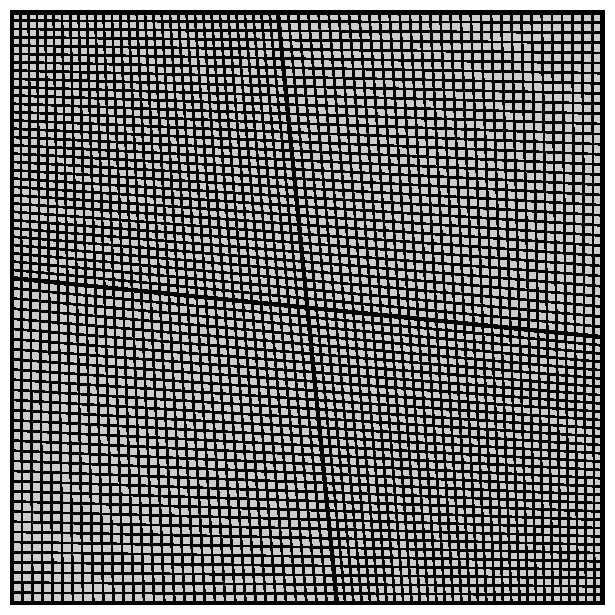
\includegraphics[scale=.431]{phase_field_domain}
		\vspace{-.4\baselineskip}
		\caption{The distorted mesh}
	\end{subfigure}
	\begin{subfigure}[t]{.3\linewidth}
		\center
		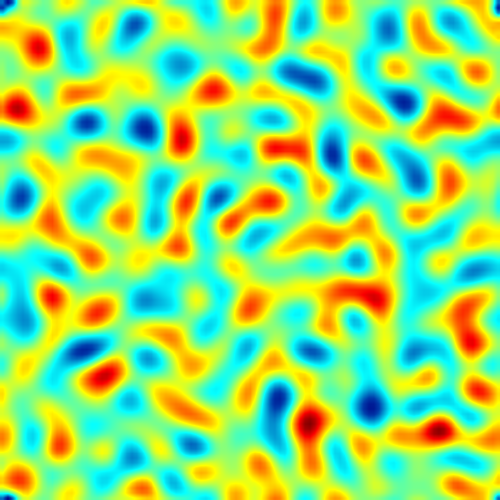
\includegraphics[scale=.25]{stochastic_ch_1_2}
		\vspace{-.4\baselineskip}
		\caption{$t=0.000002$}
	\end{subfigure}
	\begin{subfigure}[t]{.3\linewidth}
		\center
		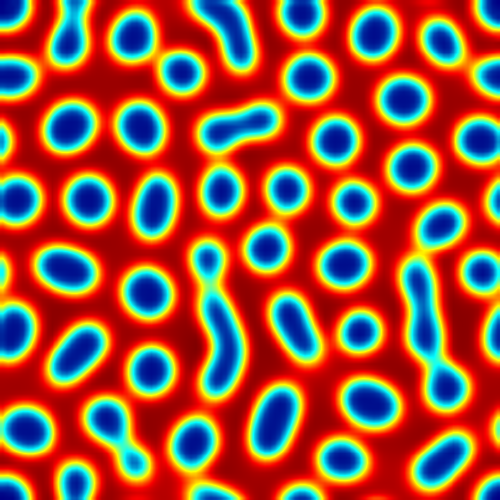
\includegraphics[scale=.25]{stochastic_ch_2_7}
		\vspace{-.4\baselineskip}
		\caption{$t=0.000007$}
	\end{subfigure}\\
	\vspace{.2\baselineskip}

	\begin{subfigure}[t]{.3\linewidth}
		\center
		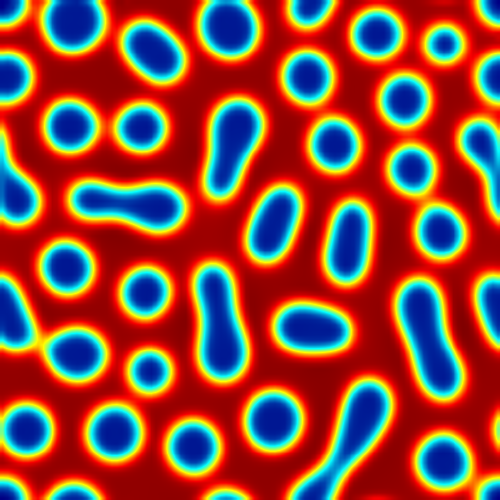
\includegraphics[scale=.25]{stochastic_ch_3_15}
		\vspace{-.4\baselineskip}
		\caption{$t=0.000015$}
	\end{subfigure}
	\begin{subfigure}[t]{.3\linewidth}
		\center
		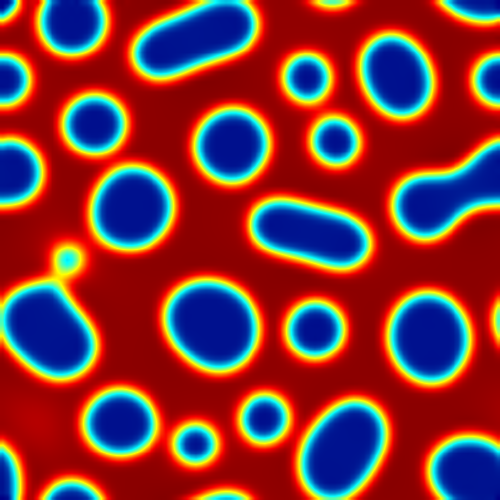
\includegraphics[scale=.25]{stochastic_ch_4_40}
		\vspace{-.4\baselineskip}
		\caption{{$t=0.000040$}}
	\end{subfigure}
	\begin{subfigure}[t]{.3\linewidth}
		\center
		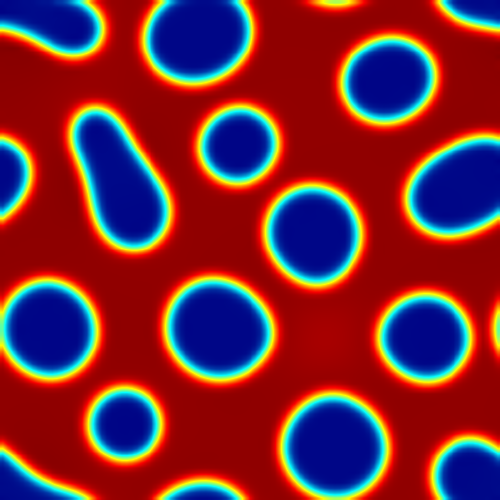
\includegraphics[scale=.25]{stochastic_ch_5_82}
		\vspace{-.4\baselineskip}
		\caption{{$t=0.000082$}}
	\end{subfigure}\\
	\vspace{.2\baselineskip}

	\begin{subfigure}[t]{.3\linewidth}
		\center
		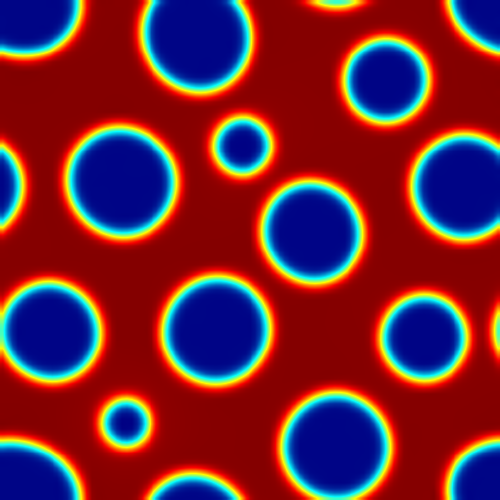
\includegraphics[scale=.25]{stochastic_ch_6_156}
		\vspace{-.4\baselineskip}
		\caption{$t=0.000156$}
	\end{subfigure}
	\begin{subfigure}[t]{.3\linewidth}
		\center
		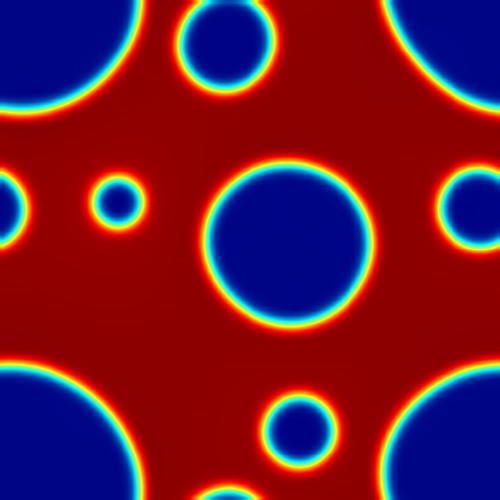
\includegraphics[scale=.25]{stochastic_ch_7_2136}
		\vspace{-.4\baselineskip}
		\caption{{$t=0.002136$}}
	\end{subfigure}
	\begin{subfigure}[t]{.3\linewidth}
		\center
		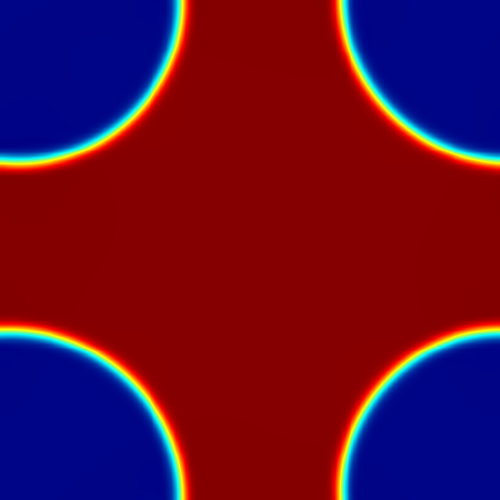
\includegraphics[scale=.25]{stochastic_ch_8}
		\vspace{-.4\baselineskip}
		\caption{Steady state}
	\end{subfigure}
	\caption{Temporal evolution of an initially stochastic concentration distribution into phases of different composition. The periodic boundary conditions are applied by the dual mortar method with the enriched dual basis. The computational domain is non-uniformly discretized, mesh lines at $\xi=0.5$ and $\eta=0.5$ are highlighted.}\label{fig:phase_field_stochastic}
\end{figure}

\subsubsection{Linear concentration distribution}

In the second case, we do not take $\bar{u}$ as a constant, but we vary it linearly with the horizontal spatial coordinate from $0.1$ to $0.9$. The domain $\Omega = \left[ 0, 2 \right] \times \left[ 0, 2 \right]$ is decomposed into four patches that are coupled non-conformingly. In addition, to show the compatibility of the coupling method with other types of boundary condition, we consider
\begin{equation}
	\frac{ \partial u}{ \partial \mathbf{n}} = 0, \;\; \text{on }\partial \Omega.
\end{equation}
This boundary condition can be incorporated into the dual mortar formulation by solving localized null space problems over each extraordinary points on the boundary.\par

The mesh and the structural evolution of the concentration distribution are demonstrated in Figure~\ref{fig:phase_field_linear}. Four patches are discretized into $63 \times 63$, $65 \times 65$, $65 \times 65$ and $63 \times 63$ cubic elements, correspondingly. In this case, three morphologies are formed in different regions of the domain. On the left-hand side of the domain, the red phase nucleates into the blue one. The exact opposite occurs on the right-hand side. In the middle, where $u\approx 0.5$, we observe the striped pattern typical from spinodal decomposition. Whereas the nucleation process is dominated in the middle region, the structural evolution at the boundaries $x = 0$ and $x = 2$ hardly exists. Eventually, the interface develops into a straight line at $x = 1$, which is consistent with the behavior of the exact solution.\par

In both cases, the convergence of the Newton's method is achieved within $3$ interations when $\Delta t<5\times 10^{-6}$ and $4$ interations when $5\times 10^{-6} \leq \Delta t < 1\times 10^{-4}$ for both the generalized-$\alpha$ method and the backward Euler method. This is the same as the simulation with one uniformly discretized patch. In addition, no influence in the time step size of the adaptive time stepping scheme has been observed. This confirms that the dual mortar method with the enriched dual basis does not impact the convergence behavior of the correction loop and the overall performance in solving nonlinear problems.

\begin{figure}[ht]
	\center
	\captionsetup[subfigure]{labelformat=empty}
	\begin{subfigure}[t]{.3\linewidth}
		\center
		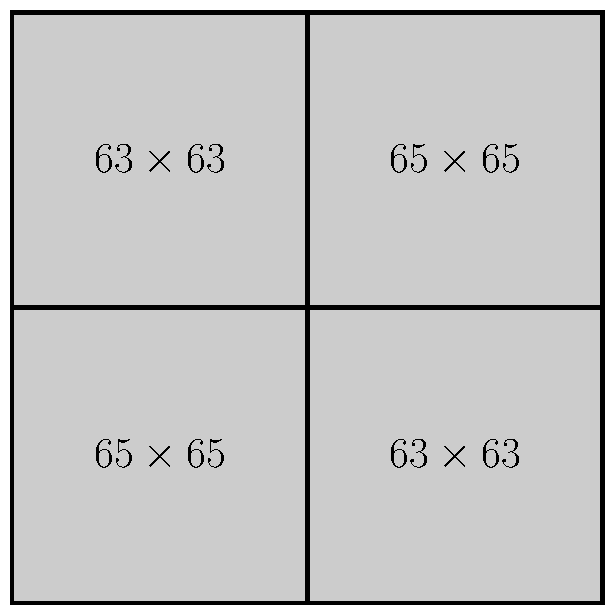
\includegraphics[scale=.431]{phase_field_domain_linear}
		\vspace{-.4\baselineskip}
		\caption{The non-conforming four-patch mesh}
	\end{subfigure}
	\begin{subfigure}[t]{.3\linewidth}
		\center
		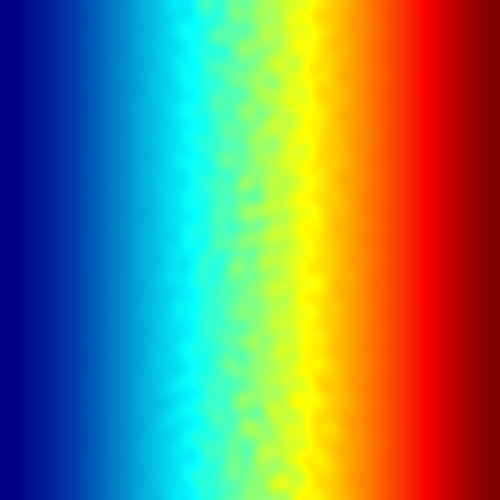
\includegraphics[scale=.25]{linear_ch_1_2}
		\vspace{-.4\baselineskip}
		\caption{$t=0.000002$}
	\end{subfigure}
	\begin{subfigure}[t]{.3\linewidth}
		\center
		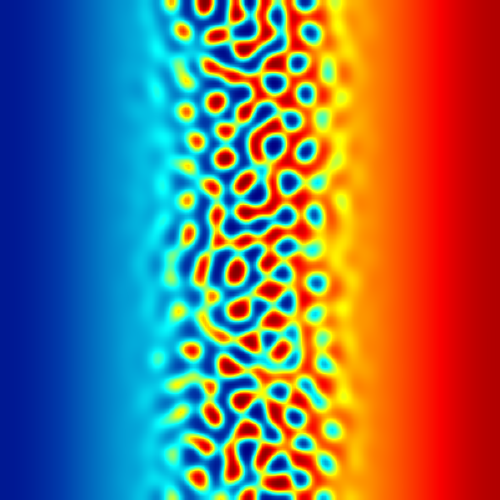
\includegraphics[scale=.25]{linear_ch_2_4}
		\vspace{-.4\baselineskip}
		\caption{$t=0.000004$}
	\end{subfigure}\\
	\vspace{.2\baselineskip}

	\begin{subfigure}[t]{.3\linewidth}
		\center
		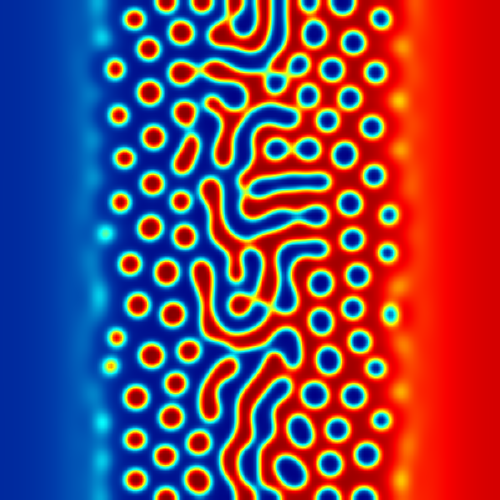
\includegraphics[scale=.25]{linear_ch_3_10}
		\vspace{-.4\baselineskip}
		\caption{$t=0.000010$}
	\end{subfigure}
	\begin{subfigure}[t]{.3\linewidth}
		\center
		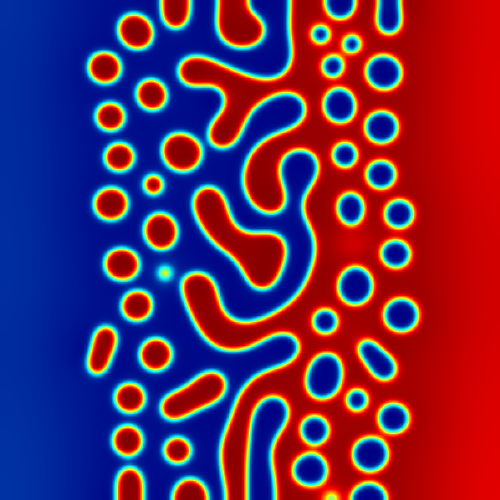
\includegraphics[scale=.25]{linear_ch_4_48}
		\vspace{-.4\baselineskip}
		\caption{{$t=0.000048$}}
	\end{subfigure}
	\begin{subfigure}[t]{.3\linewidth}
		\center
		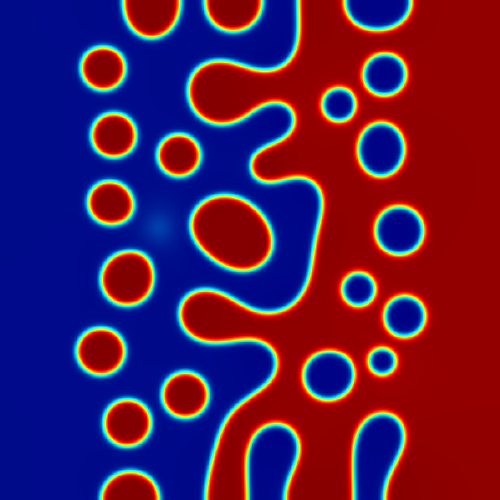
\includegraphics[scale=.25]{linear_ch_5_204}
		\vspace{-.4\baselineskip}
		\caption{{$t=0.000204$}}
	\end{subfigure}\\
	\vspace{.2\baselineskip}

	\begin{subfigure}[t]{.3\linewidth}
		\center
		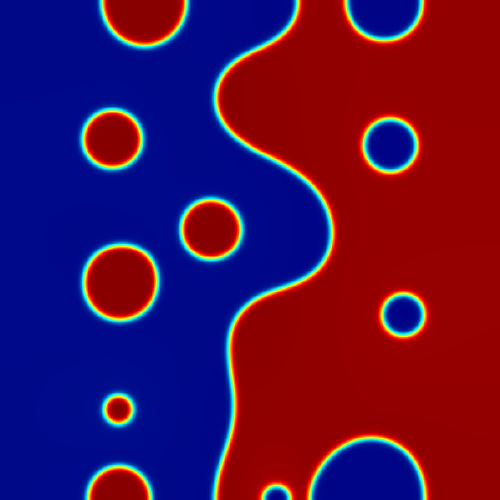
\includegraphics[scale=.25]{linear_ch_6_1304}
		\vspace{-.4\baselineskip}
		\caption{$t=0.001304$}
	\end{subfigure}
	\begin{subfigure}[t]{.3\linewidth}
		\center
		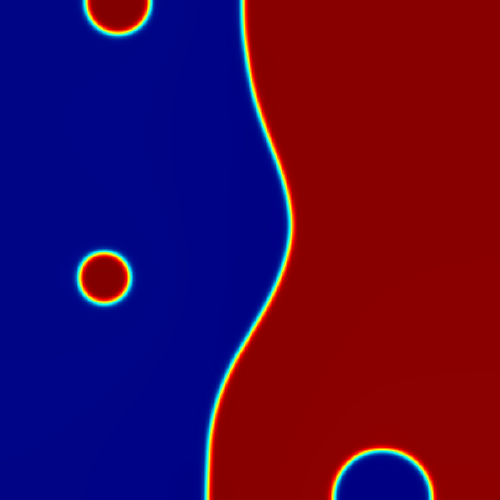
\includegraphics[scale=.25]{linear_ch_7_5814}
		\vspace{-.4\baselineskip}
		\caption{{$t=0.005814$}}
	\end{subfigure}
	\begin{subfigure}[t]{.3\linewidth}
		\center
		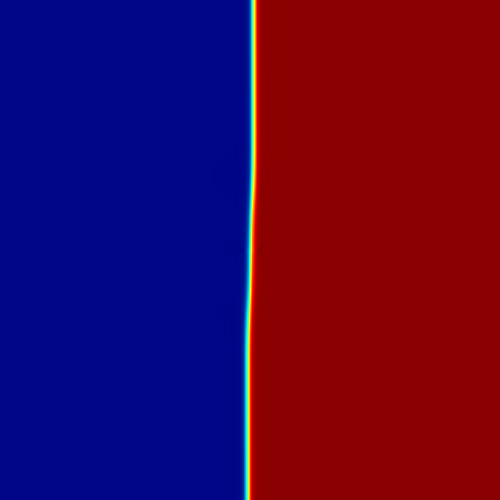
\includegraphics[scale=.25]{linear_ch_8}
		\vspace{-.4\baselineskip}
		\caption{Steady state}
	\end{subfigure}
	\caption{Temporal evolution of an initially linear concentration distribution with stochastic perturbation into two phases separated by a straight interface. The four-patch domain are coupled by the dual mortar method with the enriched dual basis.}\label{fig:phase_field_linear}
\end{figure}

\section{Conclusion}\label{sec:conlusion}

In this chapter, we develop an enrichment procedure to endow \Bezier dual basis functions with sufficient approximation ability. The cause of sub-optimal convergence of \Bezier dual basis is the lack of polynomial reproduction. The enriched \Bezier dual basis can reproduce polynomial up to a given order though at the expense of a slightly enlarged support size. Owing to the locality, the linear system from static condensation remains sparse. The proposed enrichment methodology is based on the formulation in Oswald et al.~\cite{oswald2001polynomial} and two significant improvements have been made in efficiency and robustness aspects. The proposed formulation is quadrature-free and independent of the mesh size. Hence, the cost in assembly different operators will be eliminated and the effect of the problem scale on the conditioning these operators will be minimized, giving rise to a more efficient and robust formulation. \par

The performance of the enriched \Bezier dual basis is demonstrated via several challenging benchmark problems. These problems include $2^\text{nd}$ order, $4^\text{th}$ order, linear, nonlinear, static and dynamic problems. The proposed dual basis demonstrates optimal convergence and yields compelling results as compared with the global dual basis. The robustness of the proposed dual basis is also confirmed by two highly nonlinear dynamic phase-field problems.\par

% Finally, although the proposed enrichment procedure cures the sub-optimality of \Bezier dual basis at the expense of a slightly enlarged support, we believe there exists a better formulation that can achieve the same performance without any influences on the support size. This is subjected to the future research.